%%!TEX encoding = UTF-8 Unicode 
\documentclass[english,a4paper]{report}
%%%%%%%%%%%%%%%%%%%%%%%%%%%%%%%%%%%%%%%%%%%%%%%%%%%%%%%%%%%%%%%%%%%%%%%%%%%%%%%%%%%%%%%%%%%%%%%%%%%%%%%%%%%%%%%%%%
\usepackage[portuges]{babel}
\usepackage[portuges]{minitoc}
\usepackage[utf8]{inputenc}
\usepackage[T1]{fontenc}
\usepackage[pdftex]{color,graphicx}
% pretty collors.. :)
\usepackage[a4paper, pdftex, bookmarks, colorlinks,citecolor=darkblue,linkcolor=darkblue,urlcolor=darkblue,filecolor=darkblue]{hyperref}
%\usepackage{t1enc}
%\usepackage{aeguill}
 \usepackage[avantgarde]{quotchap}
\usepackage{varioref}
\usepackage{psboxit}
\usepackage{fancybox}
\usepackage{fancyvrb}
\usepackage{color}
\usepackage{cite}
\usepackage{hyperref}
\usepackage{graphicx}
\usepackage{float}
\usepackage{listings}
\usepackage{harvard}
\usepackage{geometry}
\usepackage{graphics}
\usepackage{setspace}
\usepackage{thumbpdf}
\usepackage{fancyhdr}
\usepackage{lastpage}
\usepackage{alltt}
\usepackage{graphicx}
\usepackage{verbatim}
\usepackage{url}
\usepackage{epsf}
\usepackage{listings}
\usepackage[refpages]{gloss}
\usepackage{array}
\usepackage{longtable}
\usepackage{multirow}
\usepackage{amsmath, amsthm, amssymb}
\usepackage{slashbox}
\usepackage{rotating}
%%%%%%%%%%%%%%%%%%%%%%%%%%%%%%%%%%%%%%%%%%%%%%%%%%%%%%%%%%%%%%%%%%%%%%%%%%%%%%%%%%%%%%%%%%%%%%%%%%%%%%%%%%%%%%%%%%

\definecolor{darkblue}{rgb}{0,0.1,0.5}
%\definecolor{darkred}{rgb}{0.8,0,0}
% \def\tagform@#1{\maketag@@@{\cornersize{0.8}\ovalbox{\ignorespaces\sffamily{#1}\unskip\@@italiccorr}}}
%% first reset the headers and footers
\fancyhead{}
\fancyfoot{}
%% make the odd pages have the section name on the top right
\fancyhead[RO]{\sffamily\bfseries \rightmark}
%% make the even pages have the chapter name on the top left
\fancyhead[LE]{\sffamily\bfseries \leftmark}

%% page nums on the bottom in a nice box
%% even side pages
\fancyfoot[LE]{\psboxit{box 0.8 setgray fill}
{\framebox[10mm][c]{\rule{0cm}{4mm}\color{black}{\bfseries \thepage}}}}
%% odd side pages
\fancyfoot[RO]{\psboxit{box 1 setgray fill}
{\hspace{\textwidth}\psboxit{box 0.8 setgray fill}
{\framebox[10mm][c]{\rule{0cm}{4mm}\color{black}{\bfseries \thepage}}}}}

%% make the bottom line above the page number box
\renewcommand{\footrulewidth}{0.4pt}
\renewcommand{\footruleskip}{0mm}

\pdfpagewidth=\paperwidth
\pdfpageheight=\paperheight

\renewcommand\familydefault{\sfdefault}% usar font sem serifas

% definir acrónimos com itálico
%\renewcommand*{\acf}[1]{\acffont{\textit{\acl{#1}}~\acfsfont{(\acs{#1})}}}

\newtheorem{defin}{Definição}

\pagestyle{fancy}
%\lhead{}
%\rhead{}

%% now redefine the plain style pages (chapter pages, contents pages)
%% to have the same page number stuff on the bottom
\fancypagestyle{plain}{
	\fancyhf{}
	\fancyfoot[RO]{\psboxit{box 1 setgray fill}
	{\hspace{\textwidth}\psboxit{box 0.8 setgray fill}
	{\framebox[10mm][c]{\rule{0cm}{4mm}\color{black}{\bfseries \thepage}}}}}
	\renewcommand{\headrulewidth}{0pt}
	\renewcommand{\footrulewidth}{0.5pt}
}
% %%%%%%%%%%%%%%%%%%%%%%%%%%%%%%%%%%%%%%%%%%%%%%%%%%%%%%%%%%%%%%%%%%
\definecolor{gray_ulisses}{gray}{0.55}
\definecolor{castanho_ulisses}{rgb}{0.71,0.33,0.14}
\definecolor{preto_ulisses}{rgb}{0.41,0.20,0.04}
\definecolor{green_ulises}{rgb}{0.2,0.75,0}

%% stuff do minitoc %%%%%%%%%%%%%%%%%%%%%%%%%%%%%%%%%%%%%%%
\setcounter{minitocdepth}{2}
\setlength{\mtcindent}{24pt}
\renewcommand{\mtcfont}{\small\rm}
\renewcommand{\mtcSSfont}{\small\bf}
%\newenvironment{mtc}{\secttoc\sectlof\sectlot}{\pagebreak}
%                        ^       ^        ^
%                    conteudos  figuras  tabelas
% \newenvironment{mtc}{\minitoc\minilof\minilot}{\pagebreak}
%%%%%%%%%%%%%%%%%%%%%%%%%%%%%%%%%%%%%%%%%%%%%%%%%%%%%%%%%%%
\lstdefinelanguage{HaskellUlisses}
{
        basicstyle=\ttfamily\scriptsize,
        %backgroundcolor=\color{yellow},
        %frameshape={RYRYNYYYY}{yny}{yny}{RYRYNYYYY}, %contornos... muito nice...
        sensitive=true,
        morecomment=[l][\color{gray_ulisses}\ttfamily\tiny]{--},
        morecomment=[s][\color{gray_ulisses}\ttfamily\tiny]{\{-}{-\}},
        morestring=[b]",
        stringstyle=\color{red},
        showstringspaces=false,
%       numbers=left,
%       firstnumber=\thelstnumber,
        numberstyle=\tiny,
        numberblanklines=true,
        showspaces=false,
        breaklines=true,
        showtabs=false,
%       xleftmargin=15pt,
%       xrightmargin=-20pt,
        emph=
        {[1]
                FilePath,IOError,abs,acos,acosh,all,and,any,appendFile,approxRational,asTypeOf,asin,
                asinh,atan,atan2,atanh,basicIORun,break,catch,ceiling,chr,compare,concat,concatMap,
                const,cos,cosh,curry,cycle,decodeFloat,denominator,digitToInt,div,divMod,drop,
                dropWhile,either,elem,encodeFloat,enumFrom,enumFromThen,enumFromThenTo,enumFromTo,
                error,even,exp,exponent,fail,filter,flip,floatDigits,floatRadix,floatRange,floor,
                fmap,foldl,foldl1,foldr,foldr1,fromDouble,fromEnum,fromInt,fromInteger,fromIntegral,
                fromRational,fst,gcd,getChar,getContents,getLine,head,id,inRange,index,init,intToDigit,
                interact,ioError,isAlpha,isAlphaNum,isAscii,isControl,isDenormalized,isDigit,isHexDigit,
                isIEEE,isInfinite,isLower,isNaN,isNegativeZero,isOctDigit,isPrint,isSpace,isUpper,iterate,
                last,lcm,length,lex,lexDigits,lexLitChar,lines,log,logBase,lookup,map,mapM,mapM_,max,
                maxBound,maximum,maybe,min,minBound,minimum,mod,negate,not,notElem,null,numerator,odd,
                or,ord,otherwise,pi,pred,primExitWith,print,product,properFraction,putChar,putStr,putStrLn,quot,
                quotRem,range,rangeSize,read,readDec,readFile,readFloat,readHex,readIO,readInt,readList,readLitChar,
                readLn,readOct,readParen,readSigned,reads,readsPrec,realToFrac,recip,rem,repeat,replicate,return,
                reverse,round,scaleFloat,scanl,scanl1,scanr,scanr1,seq,sequence,sequence_,show,showChar,showInt,
                showList,showLitChar,showParen,showSigned,showString,shows,showsPrec,significand,signum,sin,
                sinh,snd,span,splitAt,sqrt,subtract,succ,sum,tail,take,takeWhile,tan,tanh,threadToIOResult,toEnum,
                toInt,toInteger,toLower,toRational,toUpper,truncate,uncurry,undefined,unlines,until,unwords,unzip,
                unzip3,userError,words,writeFile,zip,zip3,zipWith,zipWith3,listArray,doParse
        },
        emphstyle={[1]\color{blue}},
        emph=
        {[2]
                Bool,Char,Double,Either,Float,IO,Integer,Int,Maybe,Ordering,Rational,Ratio,ReadS,ShowS,String,
                Word8,InPacket
        },
        emphstyle={[2]\color{castanho_ulisses}},
        emph=
        {[3]
                case,class,data,deriving,do,else,if,import,in,infixl,infixr,instance,let,
                module,of,primitive,then,type,where
        },
        emphstyle={[3]\color{preto_ulisses}\textbf},
        emph=
        {[4]
                quot,rem,div,mod,elem,notElem,seq
        },
        emphstyle={[4]\color{castanho_ulisses}\textbf},
        emph=
        {[5]
                EQ,False,GT,Just,LT,Left,Nothing,Right,True,Show,Eq,Ord,Num
        },
        emphstyle={[5]\color{preto_ulisses}\textbf}
}
\lstnewenvironment{haskell}{\lstset{language=HaskellUlisses}}{}

\lstdefinelanguage{files} {
       basicstyle=\ttfamily\scriptsize,
       showstringspaces=false,
       showspaces=false,
       showtabs=false
}
\lstnewenvironment{code_files}{\lstset{language=files}}{}

\lstdefinelanguage{xxml} {
    basicstyle=\ttfamily\scriptsize,
	numbers=left,
	numberstyle=\tiny,
	numbersep=5pt,
	breaklines=true,
	mathescape=true,
	frame=tB
}
\lstnewenvironment{myxml}{\lstset{language=xxml}}{}

\geometry{verbose,a4paper,tmargin=30mm,bmargin=30mm,lmargin=30mm,rmargin=30mm}

%%%%%%%%%%%%%%%%%%%%%%%%%%%%%%%%%%%%%%%%%%%%%%%%%%%%%%%%%%%%%%%%%%%%%%%%%%%%%%%%%%%%%%%%%%%%%%%%%%%%%%%%%%%%%%%%%%
\begin{document}
\begin{titlepage}
\thispagestyle{empty}
\begin{figure}[htbp]
\begin{center}

\includegraphics[width=0.3\textwidth]{Images/DI-UM}
\end{center}
\end{figure}
{\centering \large
{\large\bf \textbf{Universidade do Minho} \\ Departamento de Informática}\\
\vspace{1cm}
\bf{Engenharia de Linguagens}\\
\vspace{2cm}
{\Large \bf {Projecto Integrado}}\\
\vspace{1cm}
{\LARGE \bf {\emph{Software} para Análise e Avaliação de Programas}}\\
\vspace{1cm}
%{\large \bf {}}
\vspace{8.5cm}
}

\flushleft{ \emph{Grupo 2:\\}
\vspace{0.4cm}
\begin{tabular}{ll}
José Pedro Silva & pg17628 \\
Mário Ulisses Costa & pg15817 \\
Pedro Faria & pg17684 \\
\end{tabular}
\\
}
\vspace {1.5cm}
\textbf{Braga, \today}\\
\pagebreak
\end{titlepage}

\pagenumbering{roman}
\begin{abstract}
Any traditional engineering field has metrics to rigorously assess the quality of their products.
Engineers know that the output must satisfy the requirements, must comply with the production and market rules, and must be competitive.

Professionals in the new field of software engineering started a few years ago to define metrics to appraise their product: individual programs and software systems.
This concern motivates the need to assess not only the outcome but also the process and tools employed in its development.
In this context, assessing the quality of programming languages is a legitimate objective;
in a similar way, it makes sense to be concerned with models and modeling approaches, as more and more people start the software development process by a modeling phase.

In this paper we introduce and motivate the assessment of models quality in the Software Development cycle.
After the general discussion of this topic, we focus the attention on the most popular modeling language -- the UML -- presenting metrics.
Through a Case-Study, we present and explore two tools.
To conclude we identify what is still lacking in the tools side.

%In the paper we discuss the quality of modeling languages, introducing and motivating the topic, presenting metrics, and comparing tools.
\end{abstract}
% indices
\dominitoc
\dominilof
\dominilot
\renewcommand{\contentsname}{Índice}
\tableofcontents
\addcontentsline{toc}{chapter}{\contentsname}
\renewcommand{\listfigurename}{Índice de Figuras}
\listoffigures
\addcontentsline{toc}{section}{\listfigurename}
\renewcommand{\listtablename}{Índice de Tabelas}
\listoftables
\addcontentsline{toc}{section}{\listtablename}
 

\newpage
\pagenumbering{arabic}
\addtocounter{mtc}{+2}
\newpage
\section{Introduction}
Quantitative measurements are essential in all sciences, and computer science is no exception.
Although Software Metrics aren't often used in Software Development, there has been an effort on the computer science community to develop and improve this metrics. 
The goal is to make them valuable in many aspects, such as quality assurance.\\
We present a static code analyser, that by measuring a set of metrics over C code, will give a notion of quality to the user. The software is able to generate
reports in \LaTeX~and in \textit{XML} format.\\
A system for managing programming contests, was chosen as the case study.
The competitors submit source code, which is their attempt to resolve a given problem.
The goal is not only to check if the solution is correct, but evaluate the quality of the submited code.\\
%We proceed to the next section, where we will show the system architecture, it's features and explain what is a programming contest, in this context.
%Ending with the explanation of how the parsing tree for the metrics calculation is constructed.
%We also explain the implementation of the case study, which is available in two differente plataforms.
%In the last section, we introduce the \textit{API} of the Metrics calculation, and a summarized explanation of each calculated metric.


\newpage
\part{Milestone I}
\newcommand{\rarrow}{\rightarrow}
\newcommand{\larrow}{\leftarrow}
\newcommand{\unif}{\sim}
\def\prop#1#2#3{\noindent\\$\begin{array}{l} \{#1\} \\ #2 \\ \{#3\} \\ \end{array}$\\\\}

\chapter{Modelação do Problema} \label{chap modprob}

Contextualização do cap 3

\section{Modelação Informal}\label{sec modinf}
Com o diagrama da arquitectura do sistema, figura~\ref{fig diaact},pretende-se mostrar as várias entidades que podem aceder ao sistema, assim como as várias
actividades que cada uma pode realizar e tarefas para o sistema processar.
Também é realçada a ideia de que alguns dos recursos do sistema só estão dispóniveis ao utilizador depois 
de passar por outros passos, ou seja, o diagrama dá a entender a ordem pelas quais o utilizador e o sistema podem/devem executar as tarefas.\\

\begin{figure}[htbp]
\begin{center}
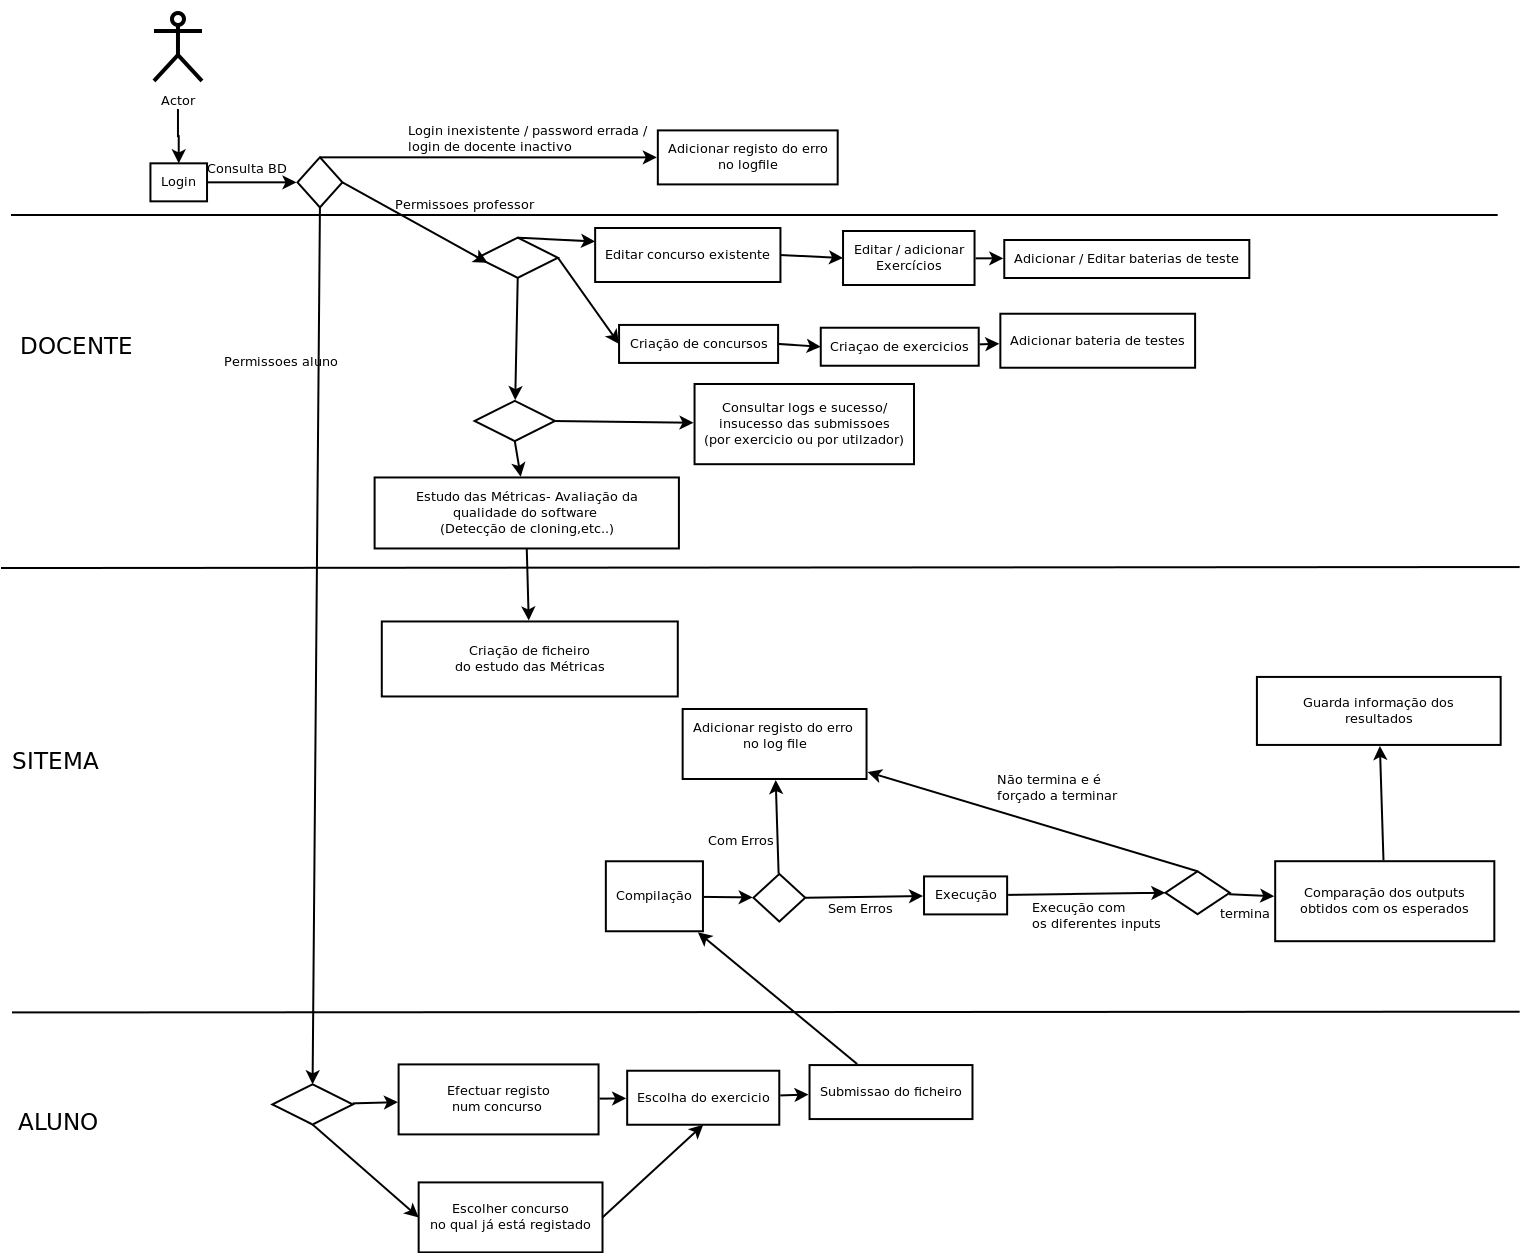
\includegraphics[width=0.9\textwidth]{Images/EL-PI}
\caption{Arquitectura do sistema}\label{fig diaact}
\end{center}
\end{figure}

Para começar, como temos duas entidades diferentes que podem aceder ao sistema (o docente e o aluno/concorrente), 
dividiu-se o diagrama em duas partes distintas (uma para cada entidade referida), de modo a facilitar a leitura.\\

Em ambos os casos, o login é a primeira actividade que pode ser realizada.
Se o login não foi efectuado com sucesso, é adicionado no log file uma entrada com a descrição do erro.
No caso de o login ser efectuado com sucesso, consoante as permissões do utilizador em questão, tem diferentes opções ao seu dispôr.\\

No caso do login pertencer a um docente, este terá acesso aos dados de cada um dos grupos, podendo verificar os resultados que estes 
obtiveram na resolução das questões do(s) concurso(s), assim como ao ficheiro que contém a análise das métricas dos vários programas submetidos 
pelos mesmos.
Poderá também criar novos concursos e os seus respectivos exercícios, assim como adicionar baterias de testes para os novos exercícios, 
ou para exercícios já existentes.\\

No caso do login pertencer a um aluno/concorrente, o utilizador terá a opção de se registar num concurso ou de seleccionar um no qual já 
esteja registado.
Já depois de seleccionar o concurso, pode ainda escolher o exercício que pretende submeter.
Depois de submeter o código fonte do programa correspondente ao exercício escolhido, e já sem a interacção do utilizador, 
o sistema compilará e tentará executar os diferentes inputs da bateria de testes do exercício, e compararar os resultados obtidos com os esperados.
No fim de cada um destes procedimentos, serão guardados os resultados / erros.
Para terminar, será feito um estudo das métricas do ficheiro submetido, tendo como resultado a criação um ficheiro com os dados relativos a essa avaliação.\\

\section{Modelação Formal}\label{sec modfor}

Afim de haver algum rigor na definição do sistema decidiu-se fazer um modelo mais formal do ponto de vista dos dados e das funcionalidades que o sistema apresenta.
A ideia desta modelação é ainda ser um modelo formal da especificação atrás descrita. Para isso utilizou-se uma notação orientada aos contratos (design by contract),
com a riqueza que as pré e pós condições de funções nos oferecem.\\

Assim sendo, temos descritos os contratos da seguinte forma:
$$\noindent\begin{array}{c} \{P\} \\ C \\ \{R\} \\ \end{array}$$
em que $P$ define uma pré condição, $C$ uma assinatura de uma função e $R$ uma pós condição.
De notar que tanto a pré como a pós condição teem de ser elementos booleanos e devem-se referir à assinatura da função. Assim sendo estamos a definir que apenas o contrato $C$
é válido se a sua pré e pós condições devolverem $true$. A pré e pós condição podem ser vazias.\\

Neste sistema que difinimos a assinatura $C$ da função pode ter uma particularidade, que é a instânciação de um elemento que pertença a um determinado tipo.
Ou seja, pode-se dizer $$soma :: a \unif Int \rarrow b \unif Int \rarrow Int$$ para expressar que a função $soma$ recebe dois parametros $a$ e $b$ que são inteiros e devolve
um elemento do tipo inteiro.\\

Decidimos, por motivos de facilidade de leitura e afim de evitar a complexidade formal, não especificar o estado interno do sistema, como por exemplo o estado do Apache,
da base de dados entre outros componentes do sistema. Achamos que especificar isso não iria trazer nada de interessante ao que pretendemos mostrar aqui.
Assim, neste modelo formal apenas se vê de forma clara, os contratos que queremos que o nosso sitema tenha.\\

Começamos então por definir o contrato da função $login$ que permite a um determinado utilizador entrar no sistema. Este contrato estipula que recebendo um par
$Username \times Hash$ e um $SessionID$ devolve ou um $Error$ ou um novo $SessionID$ que associa o utilizador à sua sessão no sistema. Afim de haver provacidade
sobre os dados criticos do utilizador, como a password, decidimos apenas receber do lado do servidor a $Hash$ respectiva da sua palavra-passe, sendo esta hash
gerada do lado do cliente. Esta técnica não tem nada de novo, mas por incrível que pareça ainda há sistemas online que não usam este tipo de mecanismos.\\

\prop
{existsInDatabase(u)}
{login :: u \unif Username \times Hash \rarrow SessionID \rarrow Error + SessionID}
{ }

Aprenta-se de seguida o modelo de dados formal que o sistema usa. Consideramos que um $Exercicio$ tem um $Enunciado$ e um dicionário a relacionar $Input's$ com $Output's$,
um concurso tem um nome, um tipo e um conjunto de exercicios.\\

$\begin{array}{l}
data~Dict~a~b = (a \times b)^{*} \\
data~Exercicio = Exercicio~Enunciado~(Dict~Input~Output) \\
data~Contest =  Contest~Nome~Tipo~Exercicio^{*}
\end{array}$\\

Para criar um novo concurso, temos de assegurar que o utilizador que requisita este serviço é um professor, visto não nos interessar que alunos criem concursos.
Temos ainda de assegurar que o concurso que se vai criar tem no minimo um exercicio.\\

\prop
{ existeSession(s)  \wedge isProf(s) \wedge (notEmpty \circ getExercice)~c}
{createContest :: s \unif SessionID \rarrow c \unif Contest \rarrow 1}
{ (notEmpty \circ getDict)~c }

Para criar um novo exercicio, o utilizador tem de ser um professor e o exercicio em questão não pode ser repetido no sistema. Decidiu-se assim para evitar redundância
na informação que se tem armazenada.

\prop
{ existeSession(s)  \wedge isProf(s) \wedge (not \circ exist) (Exercicio e d)}
{createExercice :: s\unif SessionID \rarrow e \unif Enunciado \rarrow d \unif (Dict a b) \rarrow 1}
{ exerciceCreated(Exercicio e d) }

Pode-se ainda consultar os logs de um concurso especifico. Aqui apresentamos como argumento toda o concurso - $Contest$ para apenas evitar a definição evidente
de identificadores. É claro que a implementação desta acção, irá receber como parametro o identificador do concurso, como em outros parametros deste modelo formal.

\prop 
{ existeSession(s) \wedge isProf(s) \wedge contestIsClosed(c) }
{consultarLogsContest :: s \unif SessionID \rarrow c \unif Contest \rarrow LogsContest}
{}

De seguida mostra-se a especificação de efectuar um registo no concurso, queremos apenas que o concurso não esteja cheio.

\prop
{ existSession(s) \wedge contestNotFull(c)}
{registerOnContest :: s \unif SessionID \rarrow c\unif Contest \rarrow Credenciais}
{ }

Pode-se ainda sumbmeter um exercicio, o que implica que esta acção tenha como consequência devolver um relatório com os resultados interessantes para monstrar
ao participante de um concurso.

\prop
{ existeSession(s) \wedge exerciceExist(e) }
{ submitExercicio :: s \unif SessionID \rarrow e \unif Exercicio \rarrow res \unif Resolucao \rarrow rep \unif Report}
{ rep = geraReport s e res }

\subsubsection{Modelação de acções de selecção}
Temos acções do nosso sistema que envolvem a selecção de items nos forms ou então métodos que geram efeitos secundários, assim decidimos explicar aqui esse conjunto de
contractos. Estes métodos são interessantes de modelar porque, assim fica mais claro ver os parametros que recebemos para os concretizar.\\

Temos então a acção de escolha de um exercicio numa panoplia de exercicios disponiveis no concurso que o utilizador está actualmente inscrito e a participar.\\
Relembramos que o uso do tipo $1$ significa o tipo unitário, ou seja, queremos denotar que do ponto de vista formal esta operação não devolve nada, apenas altera o sistema.
Sistema esse que no inicio explicamos que por motivos de complexidade não tinha interesse expecificar formalmente.

\prop
{ existeSession(s) \wedge exerciceExist(e) }
{escolheExercicio :: s \unif SessionID \rarrow e \unif Exercicio \rarrow 1}
{ }

Temos ainda a escolha do concurso para um grupo que está já registado.

\prop
{ existSession(s) \wedge existContest(c) \wedge userRegistadoNoContest(s,c) }
{escolheConcursoJaRegistado :: s \unif SessionID \rarrow c \unif Contest \rarrow 1}
{ }

Mostramos de seguida o contracto da função que gera um relatório ao concorrente.

\prop
{ }
{geraReport :: e \unif Exercicio \rarrow res \unif Resolucao \rarrow Report}
{ }

A titulo de exemplo, da potencialidade deste tipo de modelação, servimo-nos agora da linguagem do Haskell para especificar a definição desta operação em maior detalhe.
Temos então as seguintes definições:

\begin{eqnarray*}
geraReportBugCompile :: Exercicio \rarrow Error \rarrow Report\\
geraReportBugCompare :: Exercicio \rarrow Errado \rarrow Report\\
geraReportNoBug :: Exercicio \rarrow Resolucao \rarrow Report\\
\\
execute :: Program \rarrow Exercicio \rarrow ResolucaoProposta\\
\end{eqnarray*}

Temos ainda que $ResolucaoProposta$ é a resolução submetida pelos concorrentes e aprenstenta o seguinte tipo:

$\begin{array}{l}
data~ResolucaoProposta = Dict~Input~Output
\end{array}$\\

Temos ainda a função que recebe uma resolução como input e devolve ora um programa pronto já compilado, ora um erro no caso de surgir algum problema na compilação.

\prop
{ }
{compile :: Resolucao \rarrow Error + Program}
{ }

E ainda uma função de comparação que recebe uma resolução e um exercicio e devolve se o Output pretendido é o mesmo que o que o programa submetido origina.

\prop
{ length(Exercicio)==length(ResolucaoProposta)}
{compare :: Exercicio \rarrow ResolucaoProposta \rarrow Certo + Errado}
{ }

\begin{lstlisting}[language=HaskellUlisses]
geraReport :: Exercicio -> Resolucao -> Report
geraReport exer res = do
	case compile res of
		(Left error) -> geraReportBugCompile error res
		(Right p) ->
			let resProps = execute p exer
			in case (compare exer resProps) of
				(Left certo) -> geraReportNoBug e res
				(Right errado) -> geraReportBugCompare errado res
\end{lstlisting}

Se quisessemos este código de um ponto de vista de composição de funções a sua conversão poderia ser fácilmente atingida pelas seguintes definições:

\begin{lstlisting}[language=HaskellUlisses]
geraReport exer res =
	compile res >>= \p -> compare exer (execute p exer)
		>>= \c -> geraReportNoBug exer res
\end{lstlisting}

%geraReport e res = compile res >>= \p \rarrow compare(e (execute p e)) >>= pageCerto)

Temos ainda o contrato da função que gera o relatório final baseando-se na participação de uma equipa num determinado concurso.

\prop
{ existSession(s) \wedge existContest(c) \wedge }
{geraFinalReport :: s \unif SessionID \rarrow c \unif Contest \rarrow Dict Exercicio Resolucao \rarrow Report}
{ }

\section{Modelo de Dados}\label{sec modedados}

Definiu-se que existirão três tipos de utilizadores: o administrador, o docente e o grupo.\\

\begin{itemize}
  \item Administrador - é a entidade com mais poder no sistema. É o único que pode criar contas do tipo docente. É caracterizado por:
    \begin{itemize}
      \item Nome de utilizador;
      \item Nome completo;
      \item Password
      \item e-Mail
    \end{itemize}
  \item Docente - entidade que tem permissões para criar concursos, exercícios, aceder aos resultados das submissões, (...). 
Os seus atributos coincidem com os do Administrador.
  \item Grupo - entidade que pode registar-se em concursos e submeter tentativas para os seus diferentes enunciados.
\end{itemize}

Decidiu-se que o sistema terá a noção de grupo, e um grupo não é mais do que um conjunto de concorrentes. No entanto,
o grupo é que possui as credenciais para entrar no sistema (nome de utilizador e password). 
Além disso também tem um nome pelo qual é identificado, um e-mail que será usado no caso de haver necessidade de se entrar em contacto
com o grupo, e um conjunto de .\\

Achamos importante incluir a informação de cada concorrente no grupo para, se possível, automatizar várias tarefas tais como lançamento de notas.
Cada concorrente é caracterizado pelo seu nome completo, número de aluno (se for o caso), e e-mail.\\

\begin{figure}[htbp]
\begin{center}
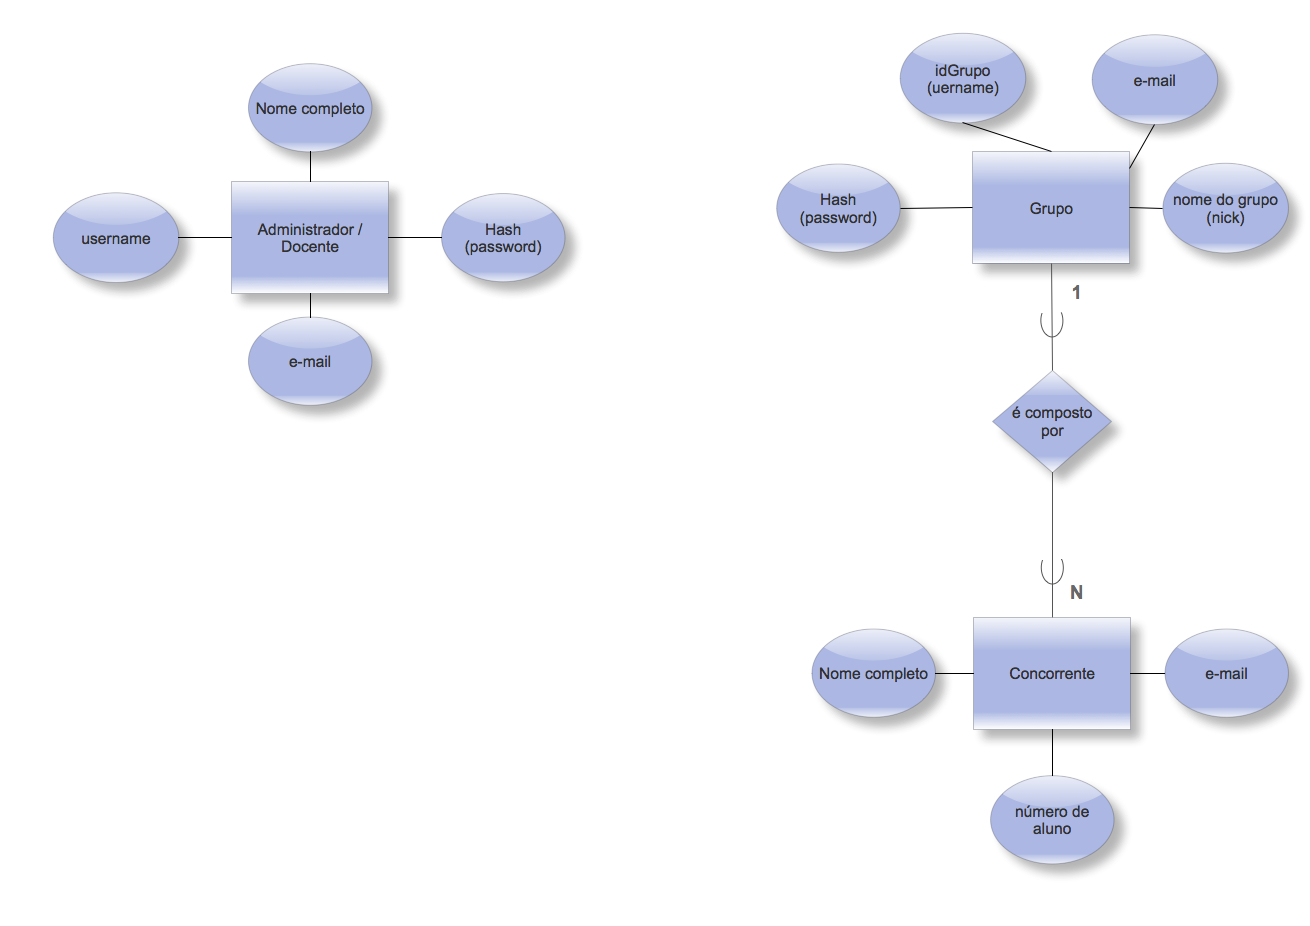
\includegraphics[width=0.9\textwidth]{Images/grupo-docente}
\caption{Modelo de dados - Grupo e Docente/Admin}\label{fig modedados-grupo-doc}
\end{center}
\end{figure}


Para finalizar vamos explicar em que consistem os concursos, enunciados e tentativas.

Um concurso, resumidamente, é um agregado de enunciados. 
Tem outras propriedades tais como um título, data de inicio e data de fim (período em que o concurso está disponível para que os grupos se registem), 
chave de acesso (necessária para o registo dos grupos), duração do concurso (tempo que o grupo tem para resolver os exercícios do concurso, 
a partir do momento que dá inicio à prova), e por fim, regras de classificação.\\
\\
Um enunciado é um exercício que o concorrente tenta solucionar. Como seria de esperar, cada exercício pode ter uma cotação diferente, 
logo o peso do enunciado é guardado no mesmo. 
Para cada enunciado existe também um conjunto de inputs e outputs, que servirão para verificar se o programa submetido está correcto. 
Contém ainda uma descrição do problema que o concorrente deve resolver, assim como uma função de avaliação, função esta que define como
 se verifica se o output obtido está de acordo com o esperado.\\
\\
Uma tentativa é a informação que é gerada pelo sistema, para cada vez que o grupo submete um ficheiro.\\
Além de conter dados sobre o concurso, enunciado e grupo a que pertence, a tentativa também contém o caminho para o código fonte do programa
submetido, data e hora da tentativa, dados referentes à compilação e um dicionário com os inputs esperados e os outputs gerados pelo programa
submetido.
\begin{figure}[htbp]
\begin{center}
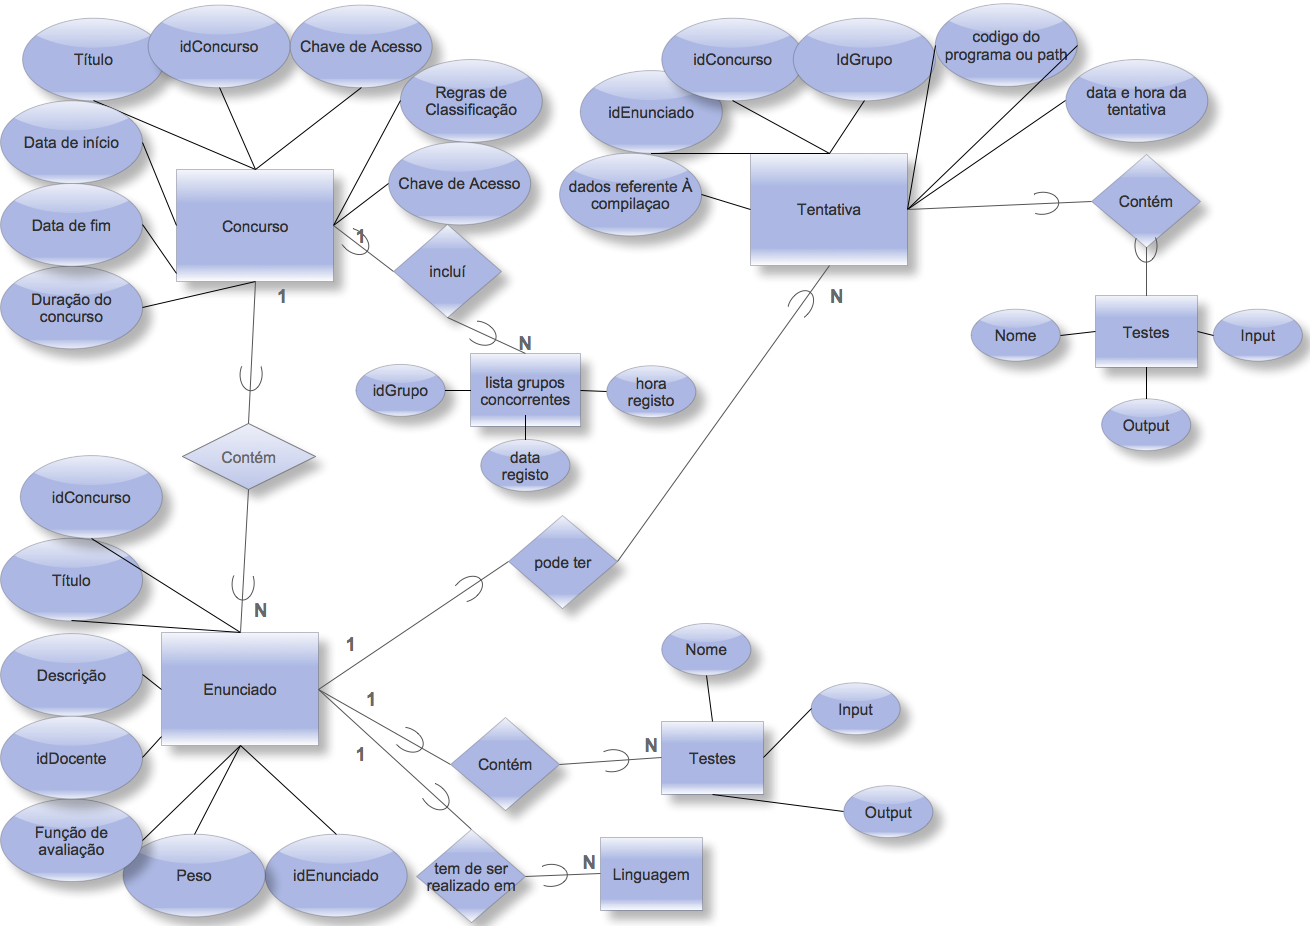
\includegraphics[width=0.9\textwidth]{Images/concurso-enunciado}
\caption{Modelo de dados - Concurso, tentativa e enunciado}\label{fig modedados-conc-enunc}
\end{center}
\end{figure}

\section{Importação de dados}\label{sec xml}

Uma das funcionalidades requeridas ao nosso sistema é a importação de enunciados e tentativas no formato xml.
Esta funcionalidade será bastante útil para demonstrar e testar o sistema, sem que se tenha de criar manualmente os enunciados
 usando a interface gráfica, ou se tenha que submeter ficheiros com código fonte, de modo a serem geradas tentativas.
Os campos presentes no xml de cada uma das entidades, \textit{enunciado} e \textit{tentativa}, são praticamente os mesmos 
que estão descritos no modelo de dados das respectivas entidades.\\
\\
No xml do enunciado, não há nada muito relevante a acrescentar, além de que não contém um id para o enunciado, pois este será gerada 
automaticamente pelo sistema. Passamos agora a apresentar um exemplo do mesmo.
\\
\lstinputlisting{resources/enunciado.xml}


Quanto ao xml para a \textit{tentativa} há que realçar o facto de que o código fonte do programa vai dentro de uma tag xml.  Além da tag xml, o código fonte
terá de ir cercado de uma secção CDATA. Isto acontece para que o que o código fonte não seja processado com o restante xml que o contém.\\
\\

\lstinputlisting{resources/tentativa.xml}


Para que todos os dados contidos nos ficheiros xml possam ser facilmente validados, foram criados dois \textit{XML schema}.
Neste schema definimos quais as tags que devem existir em cada xml, o tipo de dados e até a gama de valores que serão contido por cada tag e
 a multiplicidade das tags .\\

Nesta fase inicial do projecto ainda não foram sempre especificados  os tipos de dados que serão contidos por cada tag.\\
No entanto, para alguns dos casos em que tal aconteceu apresentaremos alguns exemplos e explicações.\\
\\
No xsd referente ao \textit{enunciado} encontramos o elemento \textit{Peso}, que é um exemplo de uma tag que contém restrições.
O \textit{Peso} terá de ser um inteiro e terá um valor entre 0 e 100.

\begin{lstlisting}
<ed:element name="Peso" default="25">
  <ed:simpleType>
    <ed:restriction base="ed:integer">
      <ed:minInclusive value="0"/>
      <ed:maxInclusive value="100"/>
    </ed:restriction>
  </ed:simpleType>
</ed:element>
\end{lstlisting}
Já o elemento \textit{Linguagem} é também restringido, mas de uma forma ligeiramente diferente. A \textit{Linguagem} será uma string, mas
apenas poderá tomar um dos valores enumerados no xsd.\\

\begin{lstlisting}
<ed:element name="Linguagem" maxOccurs="unbounded">
    <ed:simpleType>
	<ed:restriction base="ed:string">
	    <ed:enumeration value="C"/>
	    <ed:enumeration value="Java"/>
	    <ed:enumeration value="Haskell"/>
	</ed:restriction>
    </ed:simpleType>
</ed:element>
\end{lstlisting}


No xsd para a \textit{tentativa} podemos evidenciar a multiplicidade das tags, ou seja, quantas vezes algumas delas se podem repetir.
Na \textit{tentativa}, existe um \textit{Dict}, que contém uma ou mais tags \textit{Teste}.
Para definirmos que possam existir mais de que uma tag \textit{Teste} dentro de \textit{Dict}, adicionamos o atributo \textit{maxOccurs},
na entidade \textit{Teste}, com o valor \textit{``unbounded''}. O valor mínimo não é necessário definir, porque é um por default.
\begin{lstlisting}
<tt:element name="Dict">
    <tt:complexType>
	<tt:sequence>
	    <tt:element name="Teste" maxOccurs="unbounded">
		<tt:complexType>
		    <tt:sequence>
			<tt:element name="Nome" type="tt:string"/>
			<tt:element name="Input" type="tt:string"/>
			<tt:element name="Output" type="tt:string"/>
		    </tt:sequence>
		</tt:complexType>
	    </tt:element>
	</tt:sequence>
    </tt:complexType>
</tt:element>
\end{lstlisting}

Para dar uma ideia mais geral sobre ambos os \textit{xml schema} criados, em vez de apresentarmos aqui ambos os ficheiros integralmente,
vamos antes expor os diagramas que o programa \textit{oxygen} constrói e coloca ao nosso dispor, pois pensamos que torna o entendimento do
schema muito mais simples.\\
\newpage
Desta forma aqui ficam os diagramas para o enunciado e para a tentativa:\\
 
\begin{figure}[htbp]
\begin{center}
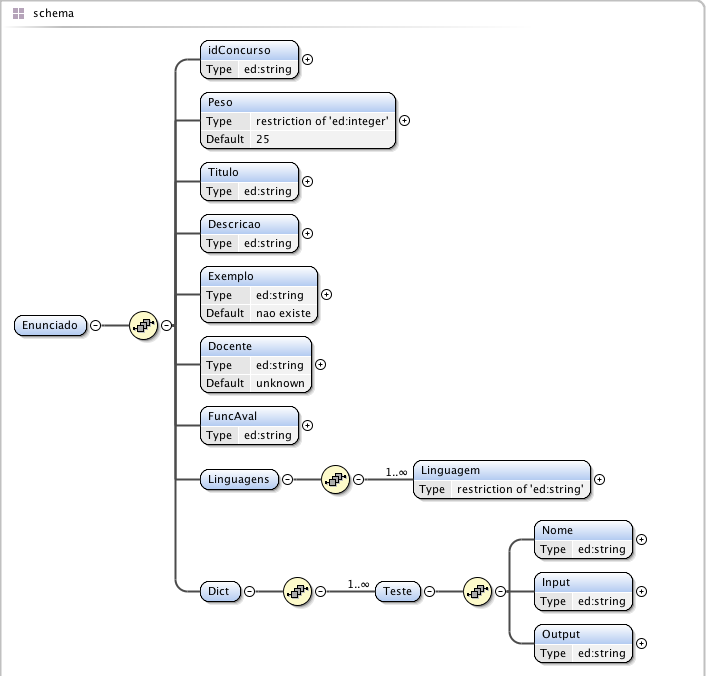
\includegraphics[width=0.9\textwidth]{Images/enunciado_schema}
\caption{diagrama do schema para o enunciado}\label{fig xsd enunciado}
\end{center}
\end{figure}

\begin{figure}[htbp]
\begin{center}
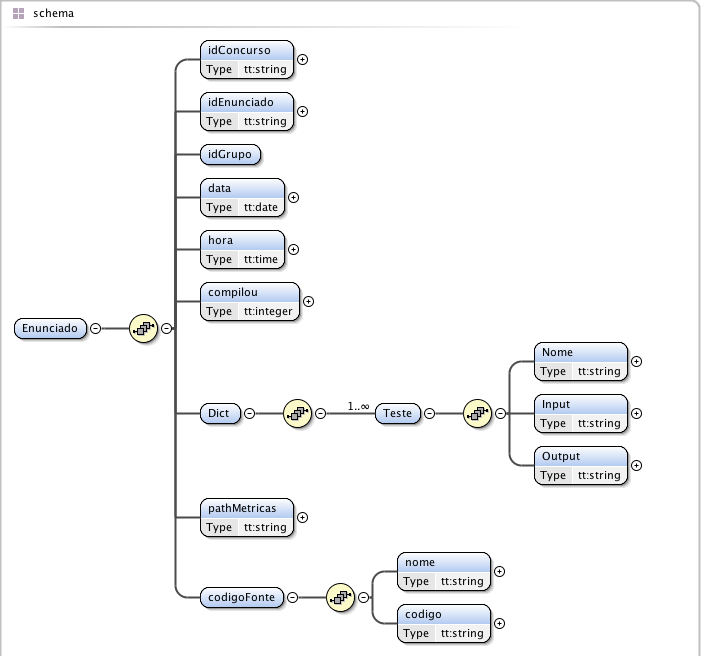
\includegraphics[width=0.9\textwidth]{Images/tentativa_schema}
\caption{diagrama do schema para a tentativa}\label{fig xsd tentativa}
\end{center}
\end{figure}

\newpage
\part{Milestone II}
\chapter{Web Application} \label{chap webApp}
\minitoc
Neste capítulo vamos expor alguns pormenores relacionados com a implementação do problema proposto.
Será explicada a maneira que encontramos para que seja seja cumprida a arquitectura que escolhemos e modelamos inicialmente.

\section{Criação de grupos, docentes e concorrentes}\label{sec gdc}
O sistema permite que qualquer utilizador não registado se registe como grupo ~\ref{img:signup}, e associe a si um ou mais concorrentes. Para efectuar o registo terá de preencher o nome do grupo/docente, um e-mail válido e uma password que tenha entre 6 a 40 caracteres.\\
Este login é utilizado por todo o grupo, para participar nos mais variados concursos.\\

\begin{figure}[H]
\begin{center}
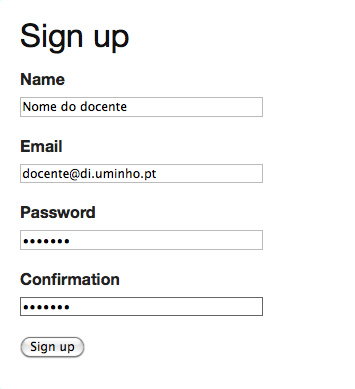
\includegraphics[width=0.45\textwidth]{Images/signup}
\caption{Página de registo}\label{img:signup}
\end{center}
\end{figure} 

Um concorrente é caracterizado por um nome, um número de aluno e um e-mail ~\ref{img:grupo}.

\begin{figure}[H]
\begin{center}
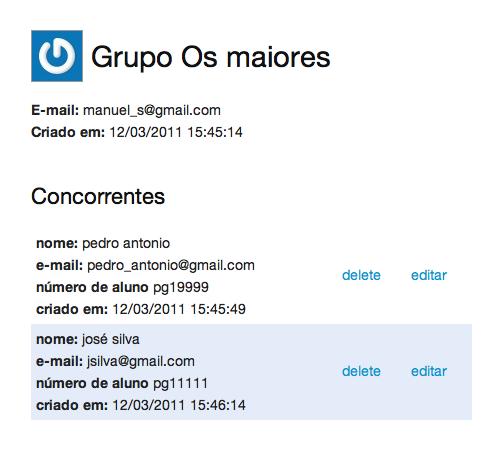
\includegraphics[scale = 0.6]{Images/grupo}
\caption{Dados de um grupo}\label{img:grupo}
\end{center}
\end{figure} 



As contas de docente só podem ser criados pelo administrador. Para simplificar o trabalho do administrador, o docente pode criar 
uma conta de grupo, à qual mais tarde será concedida privilégios de docente ~\ref{img:userToAdmin}.

\begin{figure}[H]
\begin{center}
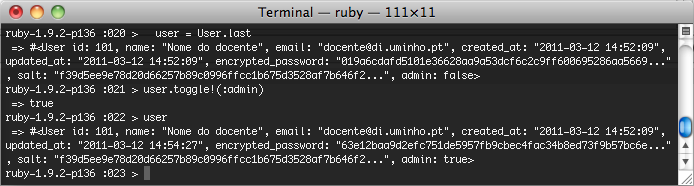
\includegraphics[scale=0.60]{Images/userToAdmin}
\caption{Comandos necessários para tornar um utilizador sem privilégios num docente.}\label{img:userToAdmin}
\end{center}
\end{figure} 

\section{Linguagens de programação}\label{sec lps}
O nosso sistema é multilingue, ou seja, é possível submeter código fonte em várias linguagens de programação diferentes, desde que 
a linguagem tenha sido correctamente configurada por um docente.
Cada linguagem é caracterizada por uma série de campos ~\ref{img:newLang}, os quais serão explicados de seguida:
\begin{itemize}
\item string de compilação: string que será executada quando se pretender compilar determinado código fonte. Esta string tem a
particularidade de no lugar em que é suposto conter o nome do ficheiro a compilar, contém \textit{\#\{file\}}.\\
Desta forma a string de compilação torna-se genérica, e independente do nome do ficheiro a compilar.
exemplo: gcc -O2 -Wall \#\{file\}

\item string simples de execução: string utilizada para executar quando o código fonte foi compilado pela string de compilação.\\
exemplo 1:\\ 
- string de compilação: gcc -O2 -Wall \#\{file\}\\
- string de execução respectiva: ./a.out\\
exemplo 2:\\
- string de compilação: gcc -O2 -Wall \#\{file\} -o exec\\
- string de execução respectiva: ./exec\\

\item string complexa de execução: a necessidade de uma segunda string de execução surgiu quando tentamos preparar o sistema para receber makefiles (inicialmente apenas para C). Nestes casos, o nome do executável gerado pela compilação não é conhecido à partida.
Desta forma é necessário analisar o makefile, e só depois executar, tendo em conta a informação que retiramos do makefile.\\
Assim, e para a linguagem C, a string complexa de execução seria:\\
- ./\#\{file\}\\
em que \#\{file\} representa o nome do executável.

\begin{figure}[H]
\begin{center}
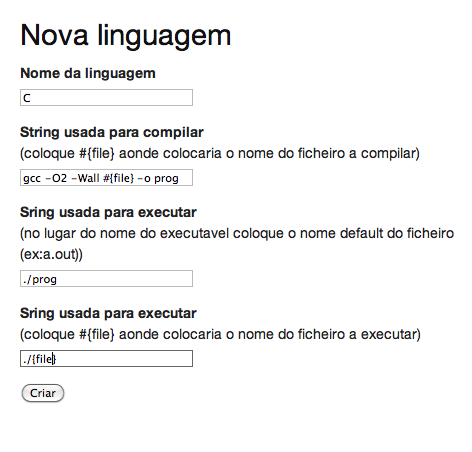
\includegraphics[scale=0.60]{Images/newLang}
\caption{Configuração de uma nova linguagem de programação no sistema}\label{img:newLang}
\end{center}
\end{figure} 

\end{itemize}

\section{Submissão de programas}\label{sec subm}
Sempre que acharem adequado, os grupos podem submeter os seus programas para serem avaliados. Para tal têm de escolher a linguagem de programação na qual resolveram o problema, de entre as disponíveis. E de seguida basta escolherem o ficheiro que pretendem submeter e carregar no botão de submissão.\\
No caso do administrador, pode ainda submeter tentativas no formato XML.

\begin{figure}[H]
\begin{center}
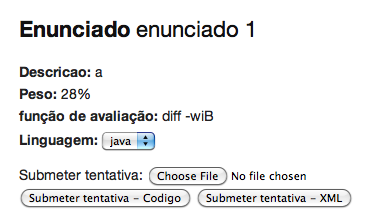
\includegraphics[scale=0.60]{Images/submissao}
\caption{Página de submissão de programas (vista de administrador)}\label{img:subm}
\end{center}
\end{figure} 

\section{Compilação}\label{sec comp}

Estando as linguagens de programação correctamente configuradas, a compilação torna-se bastante simples. Quando uma tentativa
é submetida no sistema, começamos por verificar se foi submetida apenas um ficheiro de código, ou um ficheiro comprimido.\\
Caso seja apenas um ficheiro, o sistema tenta compilar o código submetido, com a string de compilação da linguagem de programação em causa.\\
No caso de se tratar de um ficheiro comprimido, depois de o descomprimir, o sistema verifica se existe um makefile entre os ficheiros extraídos. Caso se verifique, é corrido o comando \textit{make}, e tenta retirar o nome do executável gerado, de modo a poder
ser usado na execução.

\section{Execução}\label{sec exec}
No fim da compilação, o sistema vai executar o programa uma vez para cada input. O processo de execução no caso de a compilação ter
sido feita à custa do makefile, é feita usando a string complexa de execução (sendo o nome do executável aquele que foi retirado do
makefile) . Se tal não tiver acontecido, é usada a string simples.\\
A execução pode ser abortada se ultrapassar o tempo máximo de execução, que é definido aquando da criação do enunciado em
questão. A título de demonstração, de seguida apresentamos a porção de código que "mata" o processo relativo à execução do programa,
caso ele demore mais de que o tempo máximo.

\begin{haskell}
    #thread que executa o a.out 
    out = "default";i=0
    exec = Thread.new do
      out = `#{execString} #{input}`
    end
    
    #thread que conta x segundos e dps termina a execucao do programa
    timer = Thread.new do
      sleep 5
      if exec.alive?
        Thread.kill(exec)
        i=1
        if params[:tentativa][:execStop] == false
          @erros += "Time out! Pelo menos a execucao de um dos inputs foi terminada por demorar demasiado tempo!"
        end
        params[:tentativa][:execStop] = true
      end
    end
    
    exec.join
    if timer.alive?
      Thread.kill(timer)
    end
    timer.join

\end{haskell}

\section{Guardar resultados}\label{sec res}
Para cada input do enunciado em questão, o programa é executado uma vez. O seu output é comparado com o output esperado e 
é guardada uma entrada na base de dados com a percentagem de testes nos quais o programa teve sucesso.\\
No caso de o código não compilar, ou da execução do programa demorar mais tempo do que o máximo previsto pelo docente quando 
criou o enunciado, estas informações são também guardadas na base de dados.\\
Além de se guardarem todas as tentativas, a melhor é também guardada numa tabela à parte, para que o melhor resultado para cada
enunciado seja de fácil acesso.\\
A qualquer momento o grupo pode consultar os dados relativos às suas últimas tentativas ou às últimas tentativas de todos os participantes ~\ref{img:tentativas}, e também os seus melhores resultados.\\

\begin{figure}[H]
\begin{center}
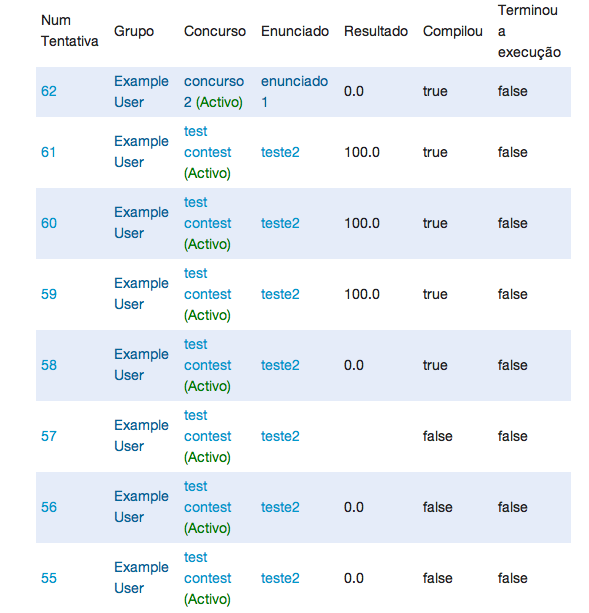
\includegraphics[scale=0.60]{Images/tentativas}
\caption{Página onde pode consultar as tentativas (vista das tentativas de todos os utilizadores)}\label{img:tentativas}
\end{center}
\end{figure}
\newpage
As métricas para avaliação de  software estão bem mais desenvolvidas que as métricas para linguagens de modelação. É então interessante ter em conta o estudo já realizado sobre métricas para avaliação de código, como é o caso das CK Metrics, como ponto de partida para métricas de modelação.\\
As CK Metrics, umas das primeiras métricas para o modelo Orientado a Objectos (OO), foram propostas por Chidamber e  Kemerer \cite{Chidamber:1994:MSO:630808.631131}. O conjunto das CK Metrics consiste em seis métricas: Weighted Methods Per Class (WMC), Depth of Inheritance Tree (DIT), Number of Children (NOC), Coupling between Object Classes (CBO), Response For a Class (RFC), e Lack of Cohesion in Methods (LCOM). Estas métricas foram depois adaptadas para linguagens de modelação. De seguida, será explicado como são calculadas cada uma das métricas referidas.

\subsection{Métricas \textrm{CK}}
\textbf{Weighted methods per class} (WMC):
Esta métrica diz respeito à complexidade que cada métodos tem para cada class. Assim, para se obter o valor desta métrica soma-se
as complexidades que cada método pertencente a uma class tem. Se considerarmos a complexidade de cada método como medida unitária
então a métrica WMC para um classe é igual ao número de métodos definidos nessa classe, referimo-nos a isto como WMC1.
A métrica WMC1 para uma classe pode ser obtida pelo diagrama de classes de um modelo UML, identificando a classe e contando o número
de métodos que essa classe implementa. Aternativamente podemos considerar a complexidade de cada método como o McCabe Cyclomatic Complexity, que referimos
como WMCcc. Os diagramas de actividade, sequencia e comunicação conteem informação relevante para o WMCcc, mas é igualmente
plausibel que os diagrama de estado possam ser usados para calcular este valor para a casse como um todo.\\

\textbf{Depth of inheritance tree} (DIT):
Esta é uma medida de profundidade da classe relativamente à sua árvore de herança. Esta métrica define-se por ser igual à distaância máxima
desde a classe até á sua super classe root na árvore de herança. Esta métrica pode ser calculada para uma classe fazendo a união de todos os diagramas
de classe num modelo \umlS e atravessando a hierarquia de herança desta classe.\\

\textbf{Number of children} (NOC): Esta métrica representa o número de decendentes imediatos de uma determinada classe. Esta métrica pode ser obtida ao juntar todos os diagramas de classes numa modelação \umlS e verificar todas as relações de herança da classe.\\

\textbf{Coupling between object classes}: Duas classes estão relacionadas se o método de uma classe usa uma variável de instância ou um método da outra classe. Uma estimativa desta métrica pode ser obtida a partir dos diagramas de classes, contando o número de classes relacionadas com a classe em questão e contando todos os tipos de referência dos atributos e todos os parâmetros dos métodos da classe. Para obter um valor mais fidedigno, pode ter em conta informação dada pelos diagramas comportamentais, de forma a obter mais informação sobre o uso das variáveis de instância e de métodos de invocação. O diagrama de sequência, por exemplo, oferece informação directa sobre interacções entre métodos de classes diferentes. \\

\textbf{Response for a class} (RFC) - esta métrica é a contagem do número de métodos que potencialmente poderão ser invocados por um objecto de uma dada classe. O número de métodos de uma classe pode ser obtido a partir de um diagrama de classes, mas o número de métodos de outras classes que são invocadas por cada um dos métodos da classe requer informação à cerca do comportamento dessa classe. Esta informação pode ser derivada a partir da inspecção de vários diagramas de comportamento (diagramas sequencias/diagramas de actividade), de modo a obter a identidade dos métodos invocados.\\


\textbf{Lack of cohesion in methods} (LCOM)- ou seja, falta de coesão entre métodos. Calcular esta métrica para uma dada classe envolve descobrir, para cada possível par de métodos, se os conjuntos de variáveis de instância acedidos por cada método têm uma interseção que não um conjunto vazio.
Para ser possível computar um valor para esta métrica, informação do modo de uso das variáveis de instância pelos métodos de uma classe é essencial. Esta informação não pode ser obtida através de uma diagrama de classes. No entanto, o valor máximo para esta métrica pode ser computado usando o número de métodos na classe. Diagramas contendo essa informação sobre o uso das variáveis, por exemplo, os diagramas sequenciais podem ser usados para calcular esta métrica.\\

O conjunto de métricas aqui definidas são referidos em vários papers e sem sombra de dúvidas são as mais estudadas, e também as mais utilizadas para avaliar modelos \uml.\\
Estas focam-se mais nos diagramas de classes visto estes serem os que mais facilmente se relacionam com código e é preciso ter em consideração que como estas regras derivam 
directamente do paradigma Orientado-a-Objectos, é mais fácil aplicá-las aos diagramas de classes. Para além disso este tipo de diagrams do ponto de vista da implementação 
dão uma visão mais geral do sistema que modela.\\
Estas métricas em particular são detalhadas por McQuillan e Power em~\cite{Power}. Também existe o SDMetrics software~\cite{SDMetrics} que avalia além destas, um conjunto
 mais extenso de métricas, que analisam outros diagramas além do de classes, como por exemplo os diagramas de estados e de actividades. \\ 
Como grande parte das métricas derivam de fórmulas matemáticas, no capítulo seguinte serão apresentadas algumas que são essenciais para o cálculo dos
valores das métricas apresentadas anteriormente.

\newpage
\chapter{Interface pelo terminal}

Tendo em vista a facilidade, para alguns utilizadores, em manusear um sistema por um terminal, decidiu-se criar uma interface para a aplicação desenvolvida. Esta interface, 
ainda em fase de desenvolvimento, vai permitir, essencialmente, trabalhar com a base de dados do sistema. Os objectivos passam por consultar listas de determinadas entidades, 
desde \texttt{enunciados} a utilizadores do sistema. De realçar que este modo de comunicação com o sistema apenas é utilizado pelos \textbf{administradores}\\

\section{Perl}

Como linguagem de desenvolvimento para esta interface, decidiu-se usar \texttt{Perl} devido à rapidez de implementação (visto que a criação de uma interface pelo terminal não 
constituía um dos principais objectivos) e a vasta diversificação de módulos existentes para auxílio ao desenvolvimento. Desses módulos, destaca-se o uso do módulo 
\texttt{DBIx::Class}, um módulo de comunicação a base de dados (apresentado durante as aulas de EL::PLN), 
que basicamente representa em classes cada tabela existente na base de dados, transformando também simples \texttt{querys} em métodos sobre as tabelas.\\

Tem-se em vista também a utilização de um módulo que use a biblioteca do sistema \texttt{Readline} e \large{Falta: readline, hash md5 para ser compativel com ruby ...}

\section{Menus e exemplos}

Na fase actual desta interface, o utilizador desta interface terá pela frente um menu principal (Figura~\ref{img menuprinc}). \\

\begin{figure}[H]
\begin{center}
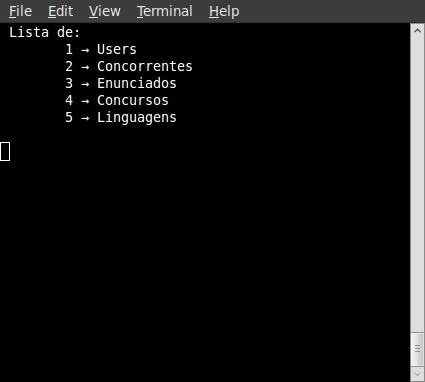
\includegraphics[width=0.45\textwidth]{Images/menuPrinc}\label{img menuprinc}
\caption{Menu Principal}
\end{center}
\end{figure} 

Cada escolha desse menu representa as principais acções que se podem efectuar com uma base de dados: 

\begin{itemize}
 \item A listagem de elementos
 \item A procura de certos elementos e posterior actualização dos mesmos
 \item A inserção de novos elementos
\end{itemize}

Assim, caso o utilizador escolha a primeira opção, será levado para um novo menu contendo as 5 principais entidades deste sistema: Os \texttt{Users}; os \texttt{Enunciados}
; os \texttt{Concorrentes}; os \texttt{Concursos}; e as \texttt{Linguagens} disponíveis para responder em cada concurso. A título de exemplo, caso o utilizador quisesse saber 
as linguagens disponíveis, a informação seria apresentada da seguinte forma(Figura~\ref{img linguagens}):\\

\begin{figure}[H]
\begin{center}
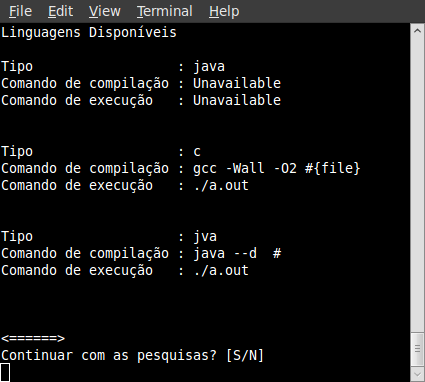
\includegraphics[width=0.45\textwidth]{Images/linguagens}\label{img linguagens}
\caption{Linguagens disponíveis}
\end{center}
\end{figure} 

O utilizador também poderia procurar por um único elemento. Como se pode ver na Figura~\ref{img zelladouglas}, dando um nome de utilizador, 
seria retornada a informação sobre esse sujeito. Caso pretendesse, o utilizador poderia posteriormente proceder à alteração do mesmo.\\

\begin{figure}[H]
\begin{center}
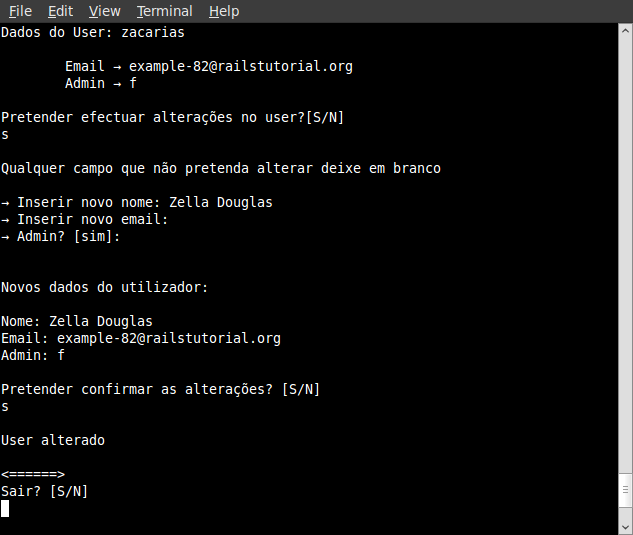
\includegraphics[width=0.65\textwidth]{Images/zacarias}\label{img zelladouglas}
\caption{Procura e alteração do \texttt{user} Zella Douglas}
\end{center}
\end{figure} 

\newpage
\chapter{Scripts de avaliação}
\minitoc

\newpage
\chapter{Front-end}
\minitoc
Como já tinhamos explicado na primeira milestone, decidimos que o nosso sistema vai tentar suportar ao máximo avaliação de métricas sobre código C.
Seria muito interessante suportar outras, mas acreditamos nesta altura que se o nosso sistema for extendido para suportar a avaliação de outras linguagens que não o C
então deveriamos recorrer a ferramentas externas que fizessem algum trabalho por nós.\\
Relativamente ao Front-end que utilizamos, ele está feito em Haskell e foi um GSoc (Google Summer of Code) feito em 2008, chama-se Language.C\footnote{Mais informação em: \url{http://trac.sivity.net/language\_c}}.
Este pacote de software apresenta um completo e bem testado parser e pretty printer para a definição da linguagem \textrm{C99} e ainda muitas das \textrm{GNU extensions}.\\

A nossa ideia é pegar em toda a investigação e trabalho dedicado à análise e descoberta de métricas, que estão descritas no Capítulo \ref{chap:metricas}, e implementa-las
utilizando este Front-end.\\

Inicialmente decidimos partir para a exploração da linguagem (dos tipos de dados) que estavam definidos neste parser. Rápidamente encontramos a AST da linguagem \textrm{C99}
e assim descobrimos que a linguagem C não é assim tão grande como estariamos à espera, como podemos ver no Apêndice \ref{chap:ast}.

\section{Estudo do Front-End}\label{chap:frontend}
Todos os tipos deste parser estão munidos de um \textrm{NodeInfo}, que nada mais é do que a informação relativa ao ficheiro, número de linha e coluna onde apareceu
esta derivação.\\
Um ficheiro em linguagem \textrm{C99} é representado como uma lista de declarações externas que pode ser uma declaração ou uma definição de função como podemos ver
na secção \ref{chap:extdefin}.

\begin{haskell}
data CTranslUnit = CTranslUnit [CExtDecl] NodeInfo
data CExtDecl = CDeclExt CDecl
              | CFDefExt CFunDef
              | CAsmExt CStrLit
\end{haskell}

Depois podemos ver que uma declaração externa pode ser então uma declaração como podemos ver na secção \ref{chap:decl}, vejamos o que é isto de declaração no \textrm{Haskell}:
\begin{haskell}
data CDecl = CDecl [CDeclSpec] [(Maybe CDeclr, Maybe CInit, Maybe CExpr)] NodeInfo
\end{haskell}
Este tipo de declarações é bastante abrangente e inclui declarações de estruturas de dados, declaração de parâmetros e tipos de dados.\\

Tal como  a definição é uma lista de declarações C e qualificadores:
\begin{haskell}
data CDeclSpec = CStorageSpec CStorageSpec  -- ^ storage-class specifier or typedef
               | CTypeSpec    CTypeSpec     -- ^ type name
               | CTypeQual    CTypeQual     -- ^ type qualifier

data CStorageSpec = CAuto     NodeInfo     -- ^ auto
                  | CRegister NodeInfo     -- ^ register
                  | CStatic   NodeInfo     -- ^ static
                  | CExtern   NodeInfo     -- ^ extern
                  | CTypedef  NodeInfo     -- ^ typedef
                  | CThread   NodeInfo     -- ^ GNUC thread local storage

data CTypeSpec = CVoidType    NodeInfo
               | CCharType    NodeInfo
               | CShortType   NodeInfo
               | CIntType     NodeInfo
               | CLongType    NodeInfo
               | CFloatType   NodeInfo
               | CDoubleType  NodeInfo
               | CSignedType  NodeInfo
               | CUnsigType   NodeInfo
               | CBoolType    NodeInfo
               | CComplexType NodeInfo
               | CSUType      CStructUnion NodeInfo  -- ^ Struct or Union specifier
               | CEnumType    CEnum        NodeInfo  -- ^ Enumeration specifier
               | CTypeDef     Ident        NodeInfo  -- ^ Typedef name
               | CTypeOfExpr  CExpr        NodeInfo  -- ^ @typeof(expr)@
               | CTypeOfType  CDecl        NodeInfo  -- ^ @typeof(type)@
\end{haskell}

\textrm{CTypeQual} diz respeito a qualificadores de tipos, por exemplo:
\begin{itemize}
\item const
\item volatile
\item restrict
\item inline
\item \_\_attribute\_\_
\end{itemize}

\begin{haskell}
data CTypeQual = CConstQual NodeInfo
               | CVolatQual NodeInfo
               | CRestrQual NodeInfo
               | CInlineQual NodeInfo
               | CAttrQual  CAttr
\end{haskell}

E ainda uma lista de triplos de \textrm{Maybe}s (Maybe CDeclr, Maybe CInit, Maybe CExpr).
Esta lista como tem 3 Maybes pode apresentar várias formas, estas formas definem o tipo de declaração que temos:

\begin{description}
\item[Toplevel declarations] Uma declaração na forma (Just declr, init?, Nothing)
\item[Structure declarations] Declarações na forma (Just declr, Nothing, size?)
\item[Parameter declarations] Declarações na forma (Just declr, Nothing, Nothing) ou (Nothing, Nothing, Just size)
\item[Toplevel declarations] Declarações na forma (Just declr, Nothing, Nothing)
\end{description}

Tempo agora para mostrar o que são estas definições \textrm{CDeclr}, \textrm{CInit} e \textrm{CExpr}.

\begin{haskell}
data CDeclr = CDeclr (Maybe Ident) [CDerivedDeclr] (Maybe CStrLit) [CAttr] NodeInfo
\end{haskell}
\textrm{CDeclr} corresponde a declarações de funções ou tipos em C. Por exemplo:

\begin{code_files}
int x;
CDeclr "x" []
\end{code_files}

\begin{code_files}
const int * const * restrict x;
CDeclr "x" [CPtrDeclr [restrict], CPtrDeclr [const]]
\end{code_files}

\begin{code_files}
int* const f();
CDeclr "f" [CFunDeclr [],CPtrDeclr [const]]
\end{code_files}

Ou seja, primeiro temos um possivel identificador, seguido de uma lista de 
declaraçõe derivadas seguido de um string literal.

Vejamos agora a definição de \textrm{CDerivedDeclr}:

\begin{haskell}
data CDerivedDeclr = CPtrDeclr [CTypeQual] NodeInfo
                   -- ^ Pointer declarator @CPtrDeclr tyquals declr@
                   | CArrDeclr [CTypeQual] (CArrSize) NodeInfo
                   -- ^ Array declarator @CArrDeclr declr tyquals size-expr?@
                   | CFunDeclr (Either [Ident] ([CDecl],Bool)) [CAttr] NodeInfo
                   -- ^ Function declarator @CFunDeclr declr (old-style-params | new-style-params) c-attrs@
\end{haskell}

Isto basicamente corresponde a uma atribuição de um pointer (CPtrDeclr attrs),
uma atribuição do resultado da computação de uma função (CFunDeclr attrs) e
atribuição de um array de elementos (CArrayDeclr attrs).

\textrm{CAttr} é simplesmente a utilização da anotação \_\_attribute\_\_

Voltando ao triplo de Maybes, temos ainda como segundo elemento \textrm{CInit} que correpondem a inicializações em C.

\begin{haskell}
data CInit = CInitExpr CExpr
             NodeInfo            -- ^ assignment expression
           | CInitList CInitList
             NodeInfo            -- ^ initialization list (see 'CInitList')
\end{haskell}
Estes inicializadoes podem ser uma de duas coisas, ou um assignment a uma expressao ou então
uma inicialização de uma lista, rodeada de parêntices de bloco.\\
Usemos então o caso das inicializações para introduzir as \textrm{CExpr}.

\begin{haskell}
data CExpr = CComma       [CExpr]       -- comma expression list, n >= 2
             NodeInfo
           | CAssign      CAssignOp     -- assignment operator
             CExpr         -- l-value
             CExpr         -- r-value
             NodeInfo
           | CCond        CExpr         -- conditional
             NodeInfo
           | CBinary      CBinaryOp     -- binary operator
             CExpr         -- lhs
             CExpr         -- rhs
             NodeInfo
           | CCast        CDecl         -- type name
             CExpr
             NodeInfo
           | CUnary       CUnaryOp      -- unary operator
             CExpr
             NodeInfo
           | CSizeofExpr  CExpr
             NodeInfo
           | CSizeofType  CDecl         -- type name
             NodeInfo
           | CAlignofExpr CExpr
             NodeInfo
           | CAlignofType CDecl         -- type name
             NodeInfo
           | CComplexReal CExpr         -- real part of complex number
             NodeInfo
           | CComplexImag CExpr         -- imaginary part of complex number
             NodeInfo
           | CIndex       CExpr         -- array
             CExpr         -- index
             NodeInfo
           | CCall        CExpr         -- function
             [CExpr]       -- arguments
             NodeInfo
           | CMember      CExpr         -- structure
             Ident         -- member name
             Bool          -- deref structure? (True for `->')
             NodeInfo
           | CVar         Ident         -- identifier (incl. enumeration const)
             NodeInfo
           | CConst       CConst        -- ^ integer, character, floating point and string constants
           | CCompoundLit CDecl
             CInitList     -- type name & initialiser list
             NodeInfo      -- ^ C99 compound literal
           | CStatExpr    CStat NodeInfo  -- ^ GNU C compound statement as expr
           | CLabAddrExpr Ident NodeInfo  -- ^ GNU C address of label
           | CBuiltinExpr CBuiltin        -- ^ builtin expressions, see 'CBuiltin'
\end{haskell}
Esta definição é tão completa que abrabge também algumas extenções feitas à linguagem C pelo, conhecidas como
GCC Extensions, como por exemplo as: alignof, \_\_real, \_\_imag, (\{ stmt-expr \}).

Terminada a explicação extensa de \textrm{CDecl}, continuamos a explicação de \textrm{CExtDecl} e passamos à definição de
\textrm{CFunDef}, ou seja uma definição de função como podemos ver em \textrm{function-definition} na secção \ref{chap:extdefin}.

\begin{haskell}
data CFunDef = CFunDef [CDeclSpec]      -- type specifier and qualifier
               CDeclr           -- declarator
               [CDecl]          -- optional declaration list
               CStat            -- compound statement
               NodeInfo
\end{haskell}

Esta definição usa uma lista de especificadores de tipo e de quantificação, uma declaração,
uma lista adicional de declarações e um C Statement. Como já explicamos todos, passamos para a explicação
do \textrm{CStat}.\\

Esta definição é capaz de ser a mais familiar e fácil de perceber na medida em que é aqui que estão
definidos os statements C que caracterizam esta linguagem:

\begin{haskell}
data CStat = CLabel  Ident CStat [CAttr] NodeInfo  -- ^ An (attributed) label followed by a statement
           | CCase CExpr CStat NodeInfo            -- ^ A statement of the form @case expr : stmt@
           | CCases CExpr CExpr CStat NodeInfo     -- ^ A case range of the form @case lower ... upper : stmt@
           | CDefault CStat NodeInfo               -- ^ The default case @default : stmt@
           | CExpr (Maybe CExpr) NodeInfo
             -- ^ A simple statement, that is in C: evaluating an expression with side-effects
             --   and discarding the result.
           | CCompound [Ident] [CBlockItem] NodeInfo    -- ^ compound statement @CCompound localLabels blockItems at@
           | CIf CExpr CStat (Maybe CStat) NodeInfo     -- ^ conditional statement @CIf ifExpr thenStmt maybeElseStmt at@
           | CSwitch CExpr CStat NodeInfo
             -- ^ switch statement @CSwitch selectorExpr switchStmt@, where @switchStmt@ usually includes
             -- /case/, /break/ and /default/ statements
           | CWhile CExpr CStat Bool NodeInfo      -- ^ while or do-while statement @CWhile guard stmt isDoWhile at@
           | CFor (Either (Maybe CExpr) CDecl)
             (Maybe CExpr)
             (Maybe CExpr)
             CStat
             NodeInfo
             -- ^ for statement @CFor init expr-2 expr-3 stmt@, where @init@ is either a declaration or
             -- initializing expression
           | CGoto Ident NodeInfo            -- ^ goto statement @CGoto label@
           | CGotoPtr CExpr NodeInfo         -- ^ computed goto @CGotoPtr labelExpr@
           | CCont NodeInfo                  -- ^ continue statement
           | CBreak    NodeInfo              -- ^ break statement
           | CReturn (Maybe CExpr)NodeInfo   -- ^ return statement @CReturn returnExpr@
           | CAsm CAsmStmt NodeInfo          -- ^ assembly statement
\end{haskell}

Aqui podemos então ver as Labels, Cases, statements de default dos Cases, expressões, ifs, switches,
whiles, fors, gotos, continues, breaks, retuns e instruções assembly.\\

Grande parte deste Front-End, Language.C, fica assim explicado. Achamos que explicar os detalhes
sobre o \textrm{CStat} não seria necessáario, visto já termos detalhado os mais importantes.

\section{Bug no \textrm{Language.C} em \textrm{MacOSX}}
Depois de explorar e usar, sempre com exemplos pequenos este front-end descobrimos que se os ficheiros C submetidos fizerem uso de biliotecas externas teriamos um
problema ao correr o avaliador de software em MacOSX. Este problema já é conhecido pela equipa que desenvolve o Language.C\footnote{Conforme se pode ver neste ticket: \url{http://trac.sivity.net/language_c/ticket/2}}.\\
Embora o nosso sistema final corra numa máquina com Linux, o desenvolvimento desta aplicação de avaliação será feito em MacOSX e assim isto confere um problema nesta fase.
Mesmo assim também foi interessante descorbrir este bug porque pretendemos que a nossa aplicação corra no máximo de plataformas possíveis. Imagine-se o caso em que
queremos rápidamente instalar numa máquina o nosso sistema para demonstração ou montar um concurso rápido, sem que seja necessário um servidor.\\

Este bug prende-se com o facto do Language.C na sua versão mais recente, 3.2.1, não suportar a notação de \_\_BLOCKS\_\_ que as librarias do MacOSX têem.\\
Imagine-se o seguinte código Haskell a usar Language.C:

\begin{haskell}
module Main where

import Language.C
import Language.C.System.GCC
import Language.C.Data.Ident
import System.Environment

process :: String -> IO ()
process file = do
    stream <- parseCFile (newGCC "gcc") Nothing [] file
    case stream of
        ( Left error  ) -> print error
        ( Right cprog ) -> print "OK"

main :: IO ()
main = do
    files <- getArgs
    mapM_ process files
\end{haskell}

O comportamento deste programa seria receber $n$ ficheiros e a cada um deles passar ao preprocessador do GCC, seguidamente é construída a árvore de parsing que fica
guardada em $stream$ e posteriormente verificamos se tivemos algum erro, se sim reportamos o erro para o $stdout$ se não então imprimimos "OK" para o $stdout$.\\

Ao alimentar este programa com o seguinte pedaço de código:

\begin{haskell}
#include <stdlib.h>

void main(int argc, char **argv) {
    malloc(10);
    return 0;
}
\end{haskell}

acontece o seguinte erro:

\begin{code_files}
[ulissesaraujocosta@maclisses:Parser]-$ ./main main.c
/usr/include/stdlib.h:272: (column 20) [ERROR]  >>> Syntax Error !
  Syntax error !
  The symbol `^' does not fit here.
\end{code_files}

Ao inspeccionar a linha 272 do stdlib.h verificamos a presença do seguinte código:

\begin{haskell}
#ifdef __BLOCKS__
int  atexit_b(void (^)(void));
void    *bsearch_b(const void *, const void *, size_t,
size_t, int (^)(const void *, const void *));
#endif /* __BLOCKS__ */
\end{haskell}

O problema reside exactamente aqui, ou seja o Language.C não consegue descobrir esta notação. Este problema parece já ter sido aberto há alguns meses e está previsto
para correcção na próxima versão 4.0 do Language.C.\\

Afim de tentarmos mesmo assim conseguir usar este front-end lembramos-nos de proibir o preprocessador do GCC para definir a variável \_\_BLOCKS\_\_. Assim sendo
temos que incluír no nosso código a injecção de uma linha de código que fará com que todos os ficheiro C processados pelo nosso programa apresentem a desactivação desta variável:

\begin{haskell}
#undef __BLOCKS__
#include <stdlib.h>

void main(int argc) {
    malloc(10);
    return 0;
}
\end{haskell}

\section{Exemplos da árvore gerada pelo Language.C}
A árvore de parsing que é criada pelo Language.C tem $84$ tipos de nodos (constructores de tipos), o que faz dela uma árvore pequena, fácil de ler, de compreender
e de começar rápidamente a trabalhar a informação contida.\\

Infelizmente o pacote Language.C não vem com as intâncias $Show$ para os tipos, o que faz com que para vermos a nossa árvore tenhamos que estar constantemente
a ler os tipos de dados e assim guiar ás escuras.\\
Assim sendo, editamos os ficheiros todos e derivamos a classe $Show$ para todos os tipos\footnote{A nossa versão do Language.C está disponível no nosso pacote de software}.\\

Agora tentamos explicar com mais detalhe relativamente à secção \ref{chap:frontend} os tipos de dados gerados pelo Language.C.\\

Imaginemos um ficheiro com o nome main.c cujo conteúdo é o seguinte:
\begin{code_files}
void lala(int a, int b);
\end{code_files}
Ou seja, apenas a declaração de uma função, depois de executar a função de parsing obtemos a seguinte árvore:
\begin{code_files}
CTranslUnit 
    [CDeclExt
        (CDecl
            [CTypeSpec (CVoidType(NodeInfo("main.c", 2, 1) (Name { nameId = 1 })))]
                [ (Just
                    (CDeclr (Just ` lala ')
                        [CFunDeclr (Right
                            ([CDecl [CTypeSpec (CIntType (NodeInfo ("main.c",2,11) (Name {nameId = 4})))]
                                [(Just (CDeclr (Just `a')[] Nothing[] (NodeInfo("main.c", 2, 15)
                                         (Name { nameId = 5 })))
                                    ,Nothing, Nothing)] (NodeInfo("main.c", 2, 11) (Name { nameId = 6 }))
                             ,CDecl [CTypeSpec(CIntType(NodeInfo("main.c", 2, 18) (Name { nameId = 8 })))]
                                 [(Just(CDeclr(Just ` b ') [] Nothing [] (NodeInfo ("main.c",2,22)
                                         (Name {nameId = 9})))
                                     ,Nothing,Nothing)]
                                 (NodeInfo ("main.c",2,18) (Name {nameId = 10}))],False))
                                 [] (NodeInfo ("main.c",2,10) (Name {nameId = 11}))
                                 ]
                                 Nothing [] (NodeInfo ("main.c",2,6) (Name {nameId = 2}))
                    )
                  ,Nothing
                  ,Nothing
                  )
                ] (NodeInfo ("main.c",2,1) (Name {nameId = 12})))]
\end{code_files}

Como podemos ver, embora a árvore de parsing seja bastante pequena, uma simples declaração de uma função
pode tomar um tamanho grande. Mesmo assim achamos bastante simples, principalmente depois de ler a especificação da AST do C.\\

Agora imaginemos que temos a seguinte função vazia em C:
\begin{code_files}
void lala(int a, int b) { }
\end{code_files}

A árvore que iríamos obter seria:
\begin{code_files}
CFDefExt
    (CFunDef
        [CTypeSpec
            (CVoidType (NodeInfo ("main.c",28,1) (Name { nameId = 71 })))
        ]
        (CDeclr
            (Just `lala')
            [CFunDeclr
                (Right
                    ([CDecl
                        [CTypeSpec(CIntType(NodeInfo("main.c", 28, 11) (Name { nameId = 74 })))]
                        [(Just(CDeclr(Just ` a ') [] Nothing
                            [] (NodeInfo ("main.c",28,15) (Name {nameId = 75})))
                        ,Nothing
                        ,Nothing)
                        ] (NodeInfo ("main.c",28,11) (Name {nameId = 76}))
                ,CDecl
                    [CTypeSpec (CIntType (NodeInfo ("main.c",28,18) (Name {nameId = 78})))]
                    [(Just (CDeclr (Just `b')[] Nothing[]
                        (NodeInfo("main.c", 28, 22) (Name { nameId = 79 })))
                        ,Nothing
                        ,Nothing)] (NodeInfo("main.c", 28, 18) (Name { nameId = 80 }))], False
                    )
                )[] (NodeInfo("main.c", 28, 10) (Name { nameId = 81 }))]
                    Nothing[] (NodeInfo("main.c", 28, 6) (Name { nameId = 72 })))[]
        (CCompound[][] (NodeInfo("main.c", 28, 25) (Name { nameId = 82 })))
            (NodeInfo("main.c", 28, 1) (Name { nameId = 83 })))
\end{code_files}


\newpage
\chapter{Conclusão e Trabalho Futuro}\label{chap con} 
Ao longo de toda primeira fase modelamos os vários aspectos do nosso sistema. Na segunda fase partimos para a implementação do
sistema e focamos também a nossa atenção na exploração de um frontend para a linguagem C.\\
\\
Toda a modelação do sistema realizada, foi importante, devido à visão mais alargada que nos deu do problema e da sua resolução.
A implementação correu de forma tranquila, onde apenas pequenos ajustes se realizaram, em relação ao pensado na fase anterior.
O trabalho relativo à importação de enunciados e tentativas em formato XML, que tinha ficado incompleto na fase I, e foi na fase II
completado.\\
O sistema está no fim desta fase apto a receber as soluções dos utilizadores, tratá-las, apresentar resultados e fazer detecção e clonning.\\
Na fase II foi também dado inicio ao desenvolvimento de uma interface em linha de comandos escrita em Perl, que alarga a acessibilidade à
aplicação, deixando do acesso à mesma estar dependente de um browser.\\
Ainda nesta fase a exploração do frontend \textit{Language.C} também deu os primeiros passos.\\
Neste momento da fase III esta ferramenta esta completamente dominada e partimos para a exploração de técnicas de programação genérica que
implemente estratégias de percorrer árvores de parsing, para conseguirmos extraír informação sobre o código que recebemos de input.
\\
Cremos que no fim desta fase III, o desenvolvimento da aplicação está terminado, foram corrigidos alguns bugs, a
interface está mais apelativa e intuitiva.\\

Para a próxima fase espera-nos o término da a aplicação pelo terminal e a aplicação de muito mais métricas e geração de um report com os resultados.


\appendix
\newpage
\chapter{AST da Linguagem \textrm{C99}}\label{chap:ast}
\minitoc
Esta definição de AST é parte da original descrita no Apendix A do K\&R\cite{ker}.
\section{Gramática Lexica}
\subsection{Elementos Lexicos}

\begin{code_files}
token:
	keyword
	identifier
	constant
	string-literal
	punctuator
preprocessing-token:
	header-name
	identifier
	pp-number
	character-constant
	string-literal
	punctuator
	each non-white-space character that cannot be one of the above
\end{code_files}

\subsection{Keywords}
\begin{code_files}
keyword:
	one of, auto, break, case, char, const
	continue, default, do, double, else
	enum, extern, float, for, goto, if
	inline, int, long, register, restrict
	return, short, signed, sizeof, static
	struct, switch, typedef, union
	unsigned, void, volatile, while
	_Bool, _Complex, _Imaginary
\end{code_files}

\subsection{Identificadores}
\begin{code_files}
identifier:
	identifier-nondigit
	identifier identifier-nondigit
	identifier digit
identifier-nondigit:
	nondigit
	universal-character-name
	other implementation-defined characters
\end{code_files}

\subsection{Universal character names}
\begin{code_files}
universal-character-name:
	\u hex-quad
	\U hex-quad hex-quad
hex-quad:
	hexadecimal-digit hexadecimal-digit
	hexadecimal-digit hexadecimal-digit
\end{code_files}

\subsection{Constantes}
\begin{code_files}
constant:
	integer-constant
	floating-constant
	enumeration-constant
	character-constant
integer-constant:
	decimal-constant integer-suffixopt
	octal-constant integer-suffixopt
	hexadecimal-constant integer-suffixopt
decimal-constant:
	nonzero-digit
		decimal-constant digit
octal-constant:
	0
	octal-constant octal-digit
hexadecimal-constant:
	hexadecimal-prefix hexadecimal-digit
	hexadecimal-constant hexadecimal-digit
hexadecimal-prefix: one of
	0x 0X
integer-suffix:
	unsigned-suffix long-suffixopt
	unsigned-suffix long-long-suffix
	long-suffix unsigned-suffixopt
	long-long-suffix unsigned-suffixopt
unsigned-suffix: one of
	u U
long-suffix: one of
	l L
long-long-suffix: one of
	ll LL
floating-constant:
	decimal-floating-constant
	hexadecimal-floating-constant
decimal-floating-constant:
	fractional-constant exponent-partopt floating-suffixopt
	digit-sequence exponent-part floating-suffixopt

hexadecimal-floating-constant:
	hexadecimal-prefix hexadecimal-fractional-constant
	binary-exponent-part floating-suffixopt
	hexadecimal-prefix hexadecimal-digit-sequence
	binary-exponent-part floating-suffixopt
fractional-constant:
	digit-sequenceopt . digit-sequence
	digit-sequence .
exponent-part:
	e signopt digit-sequence
	E signopt digit-sequence
sign: one of
	+
digit-sequence:
	digit
	digit-sequence digit
hexadecimal-fractional-constant:
	hexadecimal-digit-sequenceopt .
	hexadecimal-digit-sequence
	hexadecimal-digit-sequence .
binary-exponent-part:
	p signopt digit-sequence
	P signopt digit-sequence
hexadecimal-digit-sequence:
	hexadecimal-digit
	hexadecimal-digit-sequence hexadecimal-digit
floating-suffix: one of
	f l F L
enumeration-constant:
	identifier
character-constant:
	' c-char-sequence '
	L' c-char-sequence '

c-char-sequence:
	c-char
	c-char-sequence c-char
c-char:
	any member of the source character set except
	the single-quote ', backslash \, or new-line character
	escape-sequence
escape-sequence:
	simple-escape-sequence
	octal-escape-sequence
	hexadecimal-escape-sequence
	universal-character-name
simple-escape-sequence: one of
	\' \" \? \\
	\a \b \f \n \r \t
	\v
octal-escape-sequence:
	\ octal-digit
	\ octal-digit octal-digit
	\ octal-digit octal-digit octal-digit
hexadecimal-escape-sequence:
	\x hexadecimal-digit
	hexadecimal-escape-sequence hexadecimal-digit
\end{code_files}

\subsection{String literals}
\begin{code_files}
string-literal:
	" s-char-sequenceopt "
	L" s-char-sequenceopt "
s-char-sequence:
	s-char
	s-char-sequence s-char
s-char:
	any member of the source character set except
	the double-quote ", backslash \, or new-line character
	escape-sequence
\end{code_files}

\subsection{Header names}
\begin{code_files}
header-name:
	< h-char-sequence >
	" q-char-sequence "
h-char-sequence:
	h-char
	h-char-sequence h-char
h-char:
	any member of the source character set except
	the new-line character and >
q-char-sequence:
	q-char
	q-char-sequence q-char
q-char:
	any member of the source character set except
	the new-line character and "
\end{code_files}

\section{Phrase structure grammar}
\subsection{Expressions}
\begin{code_files}
primary-expression:
	identifier
	constant
	string-literal
	( expression )
postfix-expression:
	primary-expression
	postfix-expression [ expression ]
	postfix-expression ( argument-expression-listopt )
	postfix-expression . identifier
	postfix-expression -> identifier
	postfix-expression ++
	postfix-expression -( type-name ) { initializer-list }
	( type-name ) { initializer-list , }
argument-expression-list:
	assignment-expression
	argument-expression-list , assignment-expression
unary-expression:
	postfix-expression
	++ unary-expression
	-- unary-expression
	unary-operator cast-expression
	sizeof unary-expression
	sizeof ( type-name )
unary-operator: one of
	& * + - ~
	!
cast-expression:
	unary-expression
	( type-name ) cast-expression
multiplicative-expression:
	cast-expression
	multiplicative-expression * cast-expression
	multiplicative-expression / cast-expression
	multiplicative-expression % cast-expression

additive-expression:
	multiplicative-expression
	additive-expression + multiplicative-expression
	additive-expression - multiplicative-expression
shift-expression:
	additive-expression
	shift-expression << additive-expression
	shift-expression >> additive-expression
relational-expression:
	shift-expression
	relational-expression
	relational-expression
	relational-expression
	relational-expression
	<
	>
	<=
	>=
	shift-expression

equality-expression:
	relational-expression
	equality-expression == relational-expression
	equality-expression != relational-expression
AND-expression:
	equality-expression
	AND-expression & equality-expression
exclusive-OR-expression:
	AND-expression
	exclusive-OR-expression ^ AND-expression
inclusive-OR-expression:
	exclusive-OR-expression
	inclusive-OR-expression | exclusive-OR-expression
logical-AND-expression:
	inclusive-OR-expression
	logical-AND-expression && inclusive-OR-expression
logical-OR-expression:
	logical-AND-expression
	logical-OR-expression || logical-AND-expression
conditional-expression:
	logical-OR-expression
	logical-OR-expression ? expression : conditional-expression
assignment-expression:
	conditional-expression
	unary-expression assignment-operator assignment-expression
assignment-operator: one of
	= *= /= %= += -=
	<<= >>= &= ^= |=

expression:
	assignment-expression
	expression , assignment-expression
constant-expression:
	conditional-expression
\end{code_files}

\subsection{Declarations}\label{chap:decl}
\begin{code_files}
declaration:
	declaration-specifiers init-declarator-listopt ;
declaration-specifiers:
	storage-class-specifier declaration-specifiersopt
	type-specifier declaration-specifiersopt
	type-qualifier declaration-specifiersopt
	function-specifier declaration-specifiersopt
init-declarator-list:
	init-declarator
	init-declarator-list , init-declarator
init-declarator:
	declarator
	declarator = initializer
storage-class-specifier:
	typedef
	extern
	static
	auto
	register

type-specifier:
	void, char, short, int, long
	float, double, signed, unsigned
	_Bool, _Complex, struct-or-union-specifier
	enum-specifier, typedef-name, *

struct-or-union-specifier:
	struct-or-union identifieropt { struct-declaration-list }
	struct-or-union identifier
struct-or-union:
	struct
	union
struct-declaration-list:
	struct-declaration
	struct-declaration-list struct-declaration
struct-declaration:
	specifier-qualifier-list struct-declarator-list ;
specifier-qualifier-list:
	type-specifier specifier-qualifier-listopt
	type-qualifier specifier-qualifier-listopt
struct-declarator-list:
	struct-declarator
	struct-declarator-list , struct-declarator
struct-declarator:
	declarator
	declaratoropt : constant-expression

enum-specifier:
	enum identifieropt { enumerator-list }
	enum identifieropt { enumerator-list , }
	enum identifier
enumerator-list:
	enumerator
	enumerator-list , enumerator
enumerator:
	enumeration-constant
	enumeration-constant = constant-expression
type-qualifier:
	const
	restrict
	volatile
function-specifier:
	inline
declarator:
	pointeropt direct-declarator
direct-declarator:
	identifier
	( declarator )
	direct-declarator [ type-qualifier-listopt assignment-expressionopt ]
	direct-declarator [ static type-qualifier-listopt assignment-expression ]
	direct-declarator [ type-qualifier-list static assignment-expression ]
	direct-declarator [ type-qualifier-listopt * ]
	direct-declarator ( parameter-type-list )
	direct-declarator ( identifier-listopt )
pointer:
	* type-qualifier-listopt
	* type-qualifier-listopt pointer
type-qualifier-list:
	type-qualifier
	type-qualifier-list type-qualifier
parameter-type-list:
	parameter-list
	parameter-list , ...

parameter-list:
	parameter-declaration
	parameter-list , parameter-declaration
parameter-declaration:
	declaration-specifiers declarator
	declaration-specifiers abstract-declaratoropt
identifier-list:
	identifier
	identifier-list , identifier
type-name:
	specifier-qualifier-list abstract-declaratoropt
abstract-declarator:
	pointer
	pointeropt direct-abstract-declarator
direct-abstract-declarator:
	( abstract-declarator )
	direct-abstract-declaratoropt [ type-qualifier-listopt
	assignment-expressionopt ]
	direct-abstract-declaratoropt [ static type-qualifier-listopt
	assignment-expression ]
	direct-abstract-declaratoropt [ type-qualifier-list static
	assignment-expression ]
	direct-abstract-declaratoropt [ * ]
	direct-abstract-declaratoropt ( parameter-type-listopt )

typedef-name:
	identifier
initializer:
	assignment-expression
	{ initializer-list }
	{ initializer-list , }
initializer-list:
	designationopt initializer
	initializer-list , designationopt initializer
designation:
	designator-list =

designator-list:
	designator
	designator-list designator
designator:
	[ constant-expression ]
	. identifier
\end{code_files}

\subsection{Statements}
\begin{code_files}
statement:
	labeled-statement
	compound-statement
	expression-statement
	selection-statement
	iteration-statement
	jump-statement
labeled-statement:
	identifier : statement
	case constant-expression : statement
	default : statement
compound-statement:
	{ block-item-listopt }
block-item-list:
	block-item
	block-item-list block-item
block-item:
	declaration
	statement
expression-statement:
	expressionopt ;
selection-statement:
	if ( expression ) statement
	if ( expression ) statement else statement
	switch ( expression ) statement

iteration-statement:
	while ( expression ) statement
	do statement while ( expression ) ;
	for ( expressionopt ; expressionopt ; expressionopt ) statement
	for ( declaration expressionopt ; expressionopt ) statement
jump-statement:
	goto identifier ;
	continue ;
	break ;
	return expressionopt ;
\end{code_files}

\subsection{External definitions}\label{chap:extdefin}
\begin{code_files}
translation-unit:
	external-declaration
	translation-unit external-declaration
external-declaration:
	function-definition
	declaration
function-definition:
	declaration-specifiers declarator declaration-listopt compound-statement
declaration-list:
	declaration
	declaration-list declaration
\end{code_files}

\section{Preprocessing directives}
\begin{code_files}
preprocessing-file:
	groupopt
group:
	group-part
	group group-part
group-part:
	if-section
	control-line
	text-line
	# non-directive
if-section:
	if-group elif-groupsopt else-groupopt endif-line
if-group:
	# if
	constant-expression new-line groupopt
	# ifdef identifier new-line groupopt
	# ifndef identifier new-line groupopt
elif-groups:
	elif-group
	elif-groups elif-group
elif-group:
	# elif constant-expression new-line groupopt

else-group:
	# else new-line groupopt

endif-line:
	# endif new-line

control-line:
	# include pp-tokens new-line
	# define identifier replacement-list new-line
	# define identifier lparen identifier-listopt )
	replacement-list new-line
	# define identifier lparen ... ) replacement-list new-line
	# define identifier lparen identifier-list , ... )
	replacement-list new-line
	# undef identifier new-line
	# line pp-tokens new-line
	# error pp-tokensopt new-line
	# pragma pp-tokensopt new-line
	# new-line
text-line:
	pp-tokensopt new-line
non-directive:
	pp-tokens new-line
lparen:
	a ( character not immediately preceded by white-space
replacement-list:
	pp-tokensopt

pp-tokens:
	preprocessing-token
	pp-tokens preprocessing-token
new-line:
	the new-line character
\end{code_files}




%%%%%%%%%%%%%%%%%%%%%%%%%%%%%%%%%%%%%%%%%%%%%%%%%%%%%%%%%%%%%%%%%%%%%%%%%%%%%%%%%%%%%%%%%%%%%%%%%%%%%%%%%%%%%%%%%%
\end{document} 
